\documentclass[]{course-notes}


\title{Detailed \\ Sub--Assembly\\ Design}
\author[Gopsill et al.]{\normalsize James Gopsill, Rick Lupton, Geraint Owen \& Glen Mullineux}


\begin{document}

\maketitle

\section*{Abstract}

\begin{abstract}
    This document contains the course notes for the Detailed Sub-Assembly (shaft) design exercise. 
    In this exercise, we go through the full detailed analysis of a component and the specification of the associated components that will be attached to the component. 
\end{abstract}

\setcounter{tocdepth}{2}
\tableofcontents
\listoffigures
\listoftables

\section*{List of Acronyms}
\begin{acronym}[TDMA]
    \acro{PDS}{Product Design Specification}
    \acro{SYS}{Shear Yield Strength}
    \acro{TYS}{Tensile Yield Strength}
    \acro{USS}{Ultimate Shear Strength}
    \acro{UTS}{Ultimate Tensile Strength}
    \acro{YS}{Yield Strength}
\end{acronym}

\clearpage
\section{Introduction}

\newthought{This exercise will take you} through the detailed design and steady-state analysis of a component as well as the selection of the appropriate components to form a sub-assembly for the device. 
There is inherent uncertainty in the exercise, which you will have to overcome by making assumptions and subsequent iterations of the analysis as you begin to uncover and understand the problem that you're facing. 
This is a natural part of design and is an aspect that you will need to be able to discuss and explain within your technical design documents. 
In addition, you will be generating a list of requirements that your design needs to meet and it is highly unlikely that you will be able achieve all the desired values. 
Therefore, compromises will have to be made and you will have to highlight and discuss these within your report.

The\marginnote{Intended Learning Outcomes} Intended Learning Outcomes for this exercise are:

\begin{itemize}
    \item to practice the iterative nature of design.
    \item to develop your communication skills.
    \item to apply your 1st year engineering knowledge to a real-world problem.
    \item to record the design process you have gone through and capture your design rationale and decisions along the way.
\end{itemize}

If\marginnote{Design Process} we take a look back at our 1st year notes on the design processes, the one we're going to be focusing on in this exercise is the systematic design process model \pref{fig-vdi}.

\begin{figure}[h!]
    \centering
    \includestandalone[width=\textwidth]{01_introduction/VDI2221}
    \caption[Systematic design approach]{Systematic design approach \cite{pahl2013}}\label{fig-vdi}
\end{figure}

Some of the activities that you will be doing in this exercise are as follows:

\begin{enumerate}
    \item Product Design Specification
    \item Initial Calculations
    \item Arrangement Selection
    \item Initial Shaft Sizing
    \item Transmission Selection
    \item Bearing Selection
    \item Fixtures \& Fittings
    \item Engineering Drawing
\end{enumerate}

It is important to note that the order in which you perform these activities and where you do your iterations may be different to your peers. As a engineering designer, you will need to clearly articulate the process you have gone through to complete the exercise.

The rest of this document contains content that is pertinent to the activities you will be performing to develop a component capable of surviving the forces that it will be subjected to. Elements have also been left blank where it is expected that you perform some of your own research, attend the lectures \& tutorials to support your design work.


\clearpage
\section{Free Body Diagrams}

Free body diagrams are a method of communicating the application and direction of forces through an object. The objective is to simplify the geometry of an object to a point where one can easily see how the forces within the object interact with one another. It is also common practice to take planes in which the forces are acting to reduce the complexity of the interaction of forces further.

\cref{fig-fbd} shows an example of a loaded beam whose forces have been split in both the horizontal and vertical directions, and are reacted by two bearings. The $+$ arrow indicates our sign convention on the drawing and relative positions of the forces are also indicated.

\begin{figure*}[ht!]
    \hfill{}
    \subfloat[Vertical]{
        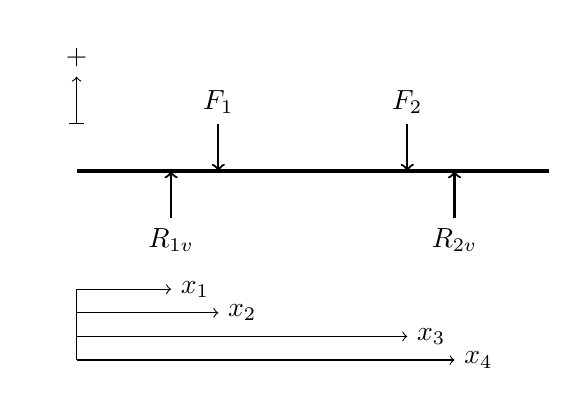
\begin{tikzpicture}[scale=6.0]
            \draw[very thick, white] (-0.1,-0.45) -- (-0.1,0.3);  % for vertical alignment with (b)
    
            \draw[very thick] (0,0) -- (1,0);
    
            \draw[<-, thick] (0.2,0) -- (0.2,-0.1) node[below]{$R_{1v}$};
            \draw[<-, thick] (0.8,0) -- (0.8,-0.1) node[below]{$R_{2v}$};
    
            \draw[<-, thick] (0.3,0) -- (0.3,0.1) node[above]{$F_{1}$};
            \draw[<-, thick] (0.7,0) -- (0.7,0.1) node[above]{$F_{2}$};
    
            \draw[->] (0,-0.25) -- (0.2,-0.25) node[right]{$x_1$};
            \draw[->] (0,-0.3) -- (0.3,-0.3) node[right]{$x_2$};
            \draw[->] (0,-0.35) -- (0.7,-0.35) node[right]{$x_3$};
            \draw[->] (0,-0.4) -- (0.8,-0.4) node[right]{$x_4$};
            \draw[] (0,-0.25) -- (0,-0.4);
    
            \draw[|->] (0,0.1) -- (0,0.2) node[above]{$+$};
        \end{tikzpicture}
    }
    \hfill{}
    \subfloat[Horizontal]{
        \begin{tikzpicture}[scale=6.0]
            \draw[very thick, white] (-0.1,-0.45) -- (-0.1,0.3); % for vertical alignment with (a)
    
            \draw[very thick] (0,0) -- (1,0);
    
            \draw[<-, thick] (0.2,0) -- (0.2,-0.1) node[below]{$R_{1h}$};
            \draw[<-, thick] (0.8,0) -- (0.8,-0.1) node[below]{$R_{2h}$};
            
            \draw[<-, thick] (0.1,0) -- (0.1,0.1) node[above]{$F_{3}$};
            
            \draw[->] (0,-0.25) -- (0.1,-0.25) node[right]{$x_0$};
            \draw[->] (0,-0.3) -- (0.2,-0.3) node[right]{$x_1$};
            \draw[->] (0,-0.35) -- (0.8,-0.35) node[right]{$x_4$};
            \draw[] (0,-0.25) -- (0,-0.35);
            
            \draw[|->] (0,0.1) -- (0,0.2) node[above]{$+$};
        \end{tikzpicture}
    }
    \hfill{}
    \vspace{2em}
    \caption{Free-body diagrams for a loaded beam}\label{fig-fbd}
\end{figure*}

Using these diagrams and information on the forces and location of the forces, one can ascertain the reactions on the bearings.

\begin{multicols}{4}
\begin{description}
    \item[$F_1$] = \SI{15}{\kilo\newton}
    \item[$F_2$] = \SI{25}{\kilo\newton}
    \item[$F_3$] = \SI{10}{\kilo\newton}
    \item[$R_{1v}$] = ?
    \item[$R_{1h}$] = ?
    \item[$R_{2v}$] = ?
    \item[$R_{2h}$] = ?
    \item[$x_0$] = \SI{0}{\metre}
    \item[$x_1$] = \SI{0.2}{\metre}
    \item[$x_2$] = \SI{0.3}{\metre}
    \item[$x_3$] = \SI{0.55}{\metre}
    \item[$x_4$] = \SI{0.6}{\metre}
\end{description}
\end{multicols}

To\marginnote{Resolving the Vertical Forces}  resolve the force vertically, we take moments about one of the bearings with the assumption that it is a static and stable system. Thus, no moment should exist about the bearing otherwise the shaft would be spinning!

Here, we have taken moments about $R_{1v}$ and from this, we can calculate the reaction force $R_{2v}$. 
\begin{align}
  \circlearrowright R_{1v} &= 0 = \SI{0.1}{\metre}(\SI{15}{\kilo\newton}) + \SI{0.35}{\metre}(\SI{25}{\kilo\newton}) - 0.4(R_{2v}) \\
  R_{2v} &= \frac{\SI{1025}{\kilo\newton\metre}}{\SI{0.4}{\metre}} = \SI{25.625}{\kilo\newton}
\end{align}

With $R_{2v}$ calculated, we can look at the balancing the forces in the vertical plane to ascertain $R_{1v}$.
\begin{align}
  R_{1v}+R_{v2}&=F_1+F_2\\
  R_{1v}+R_{v2}&=\SI{15}{\kilo\newton}+\SI{25}{\kilo\newton}\\
  R_{1v} &= \SI{40}{\kilo\newton}-\SI{25.625}{\kilo\newton} = \SI{14.375}{\kilo\newton}
\end{align}

The\marginnote{Resolving the Horizontal Forces} same process used in the horizontal direction. Taking moments about $R_{1h}$, we can find $R_{2h}$.
\begin{align}
  \circlearrowright R_{1h} &= 0 = \SI{0.2}{\metre}(\SI{10}{\kilo\newton}) + 0.4\si{\metre}(R_2) \\
  \therefore R_{2h} &=  \frac{0.2\si{\metre}}{-0.4\si{\metre}} = -5\si{\kilo\newton}
\end{align}

Again, equating the forces in the horizontal plane gives us $R_{1h}$.
\begin{align}
  R_{1h}+R_{2h}&=\SI{10}{\kilo\newton} \\
  R_{1h} &= \SI{10}{\kilo\newton} + \SI{5}{\kilo\newton} = \SI{15}{\kilo\newton}
\end{align}



\clearpage

\section{Macaulay Notation}

Macaulay Notation\footnote{N.b. This should all be familiar to you from your 1st Year Solid Mechanics.} is a method used for the structural analysis of Euler-Bernoulli beams and describes the beam forces, moments and deflection. The method is particularly useful for discontinuous and/or discrete loading scenarios as well as loadings that are uniformly distributed loads (u.d.l.) and/or uniformly varying loads (u.v.l.) over the span of a beam.

The\marginnote{Method} method starts with the Euler-Bernoulli beam theory and the relation between the deflection $w$ and bending moment $M$.

\begin{equation}
  \pm EI\frac{\text{d}^2 w}{\text{d}x^2} = M
\end{equation}

\noindent Where $E$ is the elastic modulus and $I$ is the second moment of area.

In terms of Macaulay Notation, $M$ is expressed in the form:

\begin{equation}
  M = M_1(x) + P_1\langle x-a_1\rangle^{b_1} + P_2\langle x-a_2\rangle^{b_2} + P_3\langle x-a_3\rangle^{b_3} + \ldots
\end{equation}

\noindent Where $M_1$ is the moment at the start of $x$ and $P_i\langle x-a_i\rangle^{b_i}$ representing elements along the beam that contribute to the moment. These contribute to the scenario when $x$ becomes greater than $a_i$:

\begin{equation}
  \langle x - a_i\rangle = 
  \begin{cases} 
    0 & \mathrm{if}~ x < a_i \\ 
    x - a_i & \mathrm{if}~ x > a_i 
  \end{cases}
\end{equation}

\noindent $b_i$ is determined by the type of loading that is being applied. 

For\marginnote{Shear Force} the shaft design exercise, you will be taking the shear forces and integrating them to get your bending moments for the two axes. For example, the Macaulay Notation for the Free Body Diagrams in \cref{fig-fbd} are as follows:
\begin{equation}
  S_v = R_{v1}\langle x-x_1\rangle^0 + F_{1}\langle x-x_2\rangle^0  + F_{2}\langle x-x_3\rangle^0 + R_{v2}\langle x-x_4\rangle^0
\end{equation}
\begin{equation}
  S_h = F_{3}\langle x-x_0\rangle^0 + R_{h1}\langle x-x_2\rangle^0 + R_{h2}\langle x-x_4\rangle^0
\end{equation}

From\marginnote{Shear Force Diagram} these equations, the shear force diagrams for the two axes can be generated (\cref{fig-sfd}).

\begin{figure*}[th!]
    
    \hfill
    \subfloat[Vertical Shear]{
        \includestandalone[width=0.45\textwidth, mode=buildnew]{03_macaulay_notation/vertical_shear}
    }
    \hfill
    \subfloat[Horizontal Shear]{
        \includestandalone[width=0.45\textwidth, mode=buildnew]{03_macaulay_notation/horizontal_shear}
    }
    \hfill
    
    \vspace{2em}
    \caption{Shear force diagrams}
    \label{fig-sfd}
\end{figure*}


Having\marginnote{Bending Moment}  described the shear forces in Macaulay Notation, it is then the case of integrating and determining the constant of integration to arrive at an equation that describes the bending moment at any point through the beam.
\begin{equation}
  M_v = \int S_v = R_{v1}\langle x-x_1\rangle^1 + F_{1}\langle x-x_2\rangle^1  + F_{2}\langle x-x_3\rangle^1 + R_{v2}\langle x-x_4\rangle^1
\end{equation}
\begin{equation}
  M_h = \int S_h = F_{3}\langle x-x_0\rangle^1 + R_{h1}\langle x-x_2\rangle^1 + R_{h2}\langle x-x_4\rangle^1
\end{equation}

Using\marginnote{Bending Moment Diagram} these equations, one can obtain the bending moment diagrams for the loaded beam (\cref{fig-bmd}).

\begin{figure*}[th!]

    \hfill
    \subfloat[Vertical Bending]{
        \includestandalone[width=0.45\textwidth, mode=buildnew]{03_macaulay_notation/vertical_bending}
    }
    \hfill
    \subfloat[Horizontal Bending]{
        \includestandalone[width=0.45\textwidth, mode=buildnew]{03_macaulay_notation/horizontal_bending}
    }
    \hfill
    
    \vspace{2em}
    \caption{Bending Moment Diagrams}\label{fig-bmd}
\end{figure*}


\clearpage
\section{Failure Modes of Shafts}

\newthought{There are a number of shaft failure modes} and it is important to recognise the types of failure that can occur and be able to perform the subsequent analysis to mitigate this occurring within our design. It is up to you to do some research on the types of failure and to discuss the failures that might occur for your shaft. Whilst this section does not detail the types of failure, it does provide the calculations required to determine the stresses within the shaft so that you will be able to evaluate whether the shaft will survive the forces that it is being subjected to.

\subsection{Types of Failure}

\begin{framed}
    \vspace{1cm}
    \begin{center}
        \Large
        -- Own Research \& Lectures --
    \end{center}
    \vspace{1cm}
\end{framed}

\subsection{Calculating Shaft Stresses}

\marginnote{Direct Stress $(\sigma_d)$} The first is the direct stress acting through the cross-section of the shaft.
If the shaft diameter is not large enough then shaft will simply shear as if one were creating a cross-section through the shaft.
The Direct Stress is given by \cref{equ-direct-stress}.

\begin{equation}
    \sigma_d = \frac{F}{A}
    \label{equ-direct-stress}
\end{equation}

However, it is very rare for a shaft to fail through Direct Stress through the shafts cross-section. It is more likely that a shaft will fail due to the combined bending, hoop and torsional stresses acting on the outer surface of the shaft, which can be resolved using Mohr's Circle \mycite{clifford2012}.

Taking\marginnote{Mohr's circle}  a 2D element on the outer surface of the shaft, the bending, hoop and torsional stresses can be related as shown in \cref{fig-mohrs-circle}. Where $\sigma_x$ is the bending stress, $\sigma_y$ is the hoop stress and $\tau_{xy}$ is the torsional stress.

\begin{marginfigure}
    \centering
    \includestandalone[width=0.8\textwidth, mode=buildnew]{04_failure_modes/mohrs-circle}
    \caption{2D mohr's circle}
    \label{fig-mohrs-circle}
\end{marginfigure}

Bending\marginnote{Bending Stress $(\sigma_x)$}  stress is the Direct Stress in the direction of the axis of the shaft and is due to the bending moment. This can be calculated using Equation~\ref{equ-bending-stress}.

\begin{equation}
    \sigma_{x} = \frac{My}{I}
    \label{equ-bending-stress}
\end{equation}

Where $I$ is the Second Moment of Area:

\begin{equation}
    I = \frac{\pi r^4}{4}
\end{equation}

Hoop\marginnote{Hoop Stress \(\sigma_y\)} stress is the direct stress due to forces attempting to expand the shaft. This is only really the case when considering pressure vessels where the interior pressure of the gas or liquid is wanting to expand the vessel. In our cases, we can say that \(\sigma_y = 0\). 

Torsional\marginnote{Torsional Stress \(\tau_{xy}\)} stress is the shear stress due to torsion (twisting) and can by calculated using Equation~(\ref{equ:torsional-stress}).

\begin{equation}
    \tau_{xy} = \frac{Tr}{J}
    \label{equ:torsional-stress}
\end{equation}

Where \(J\) is the Polar Moment of Area:

\begin{equation}
    J = \frac{\pi d^4}{32}
\end{equation}

These stress depend upon the orientation of the element. If another element is taken, twisted through an angle \(\phi\), as shown in Figure, then the Direct Stresses are \(\sigma_x\) and \(\sigma_X\) and the shear stress is \(\tau_{xy}\) = \(\tau_{XY}\). And these are normally different from the first set of stresses in \cref{fig-rotated-mohrs-circle}.

\begin{marginfigure}
    \centering
    \includestandalone[width=0.8\textwidth, mode=buildnew]{04_failure_modes/mohrs-circle-rotated}
    \caption{Mohr's circle rotated by \(\phi\)}
    \label{fig-rotated-mohrs-circle}
\end{marginfigure}

The two sets of stresses are related by formulae involving the sine and cosine of twice the angle, 2\(\phi\). Mohr's circle is a graphical way of representing these formulae. The construction of the circle is as follows and is shown in \cref{fig-m-circle}.

\begin{enumerate}
    \item Draw the line AB between points with coordinates: \(\text{A} = (\sigma_x, -\tau_{xy}) \) and \(\text{B} = (\sigma_y, \tau_{xy}) \)
    \item Draw the circle with AB as diameter
\end{enumerate}

\begin{figure}[h!]
    \includestandalone[width=\textwidth, mode=buildnew]{04_failure_modes/m-circle}
    \caption{Mohr's circle relating stresses associated with elements with different orientations}
    \label{fig-m-circle}
\end{figure}

Then, to find the stresses related to the element rotated through angle \(\phi\), the diameter AB is rotated through angle \(2\phi\), giving diameter CD. The positions of C and D give the other stress with: \(\text{C} = (\sigma_X, -\tau_{XY}) \) and \(\text{D} = (\sigma_Y, \tau_{XY}) \).

Mohr's\marginnote{Principal Stresses} circle shows there are two special cases. The first is when the diameter AB is rotated so that it becomes horizontal. The corresponding element undergoes no shear stress, but is subject to two direct stresses (in perpendicular directions) which are \(\sigma_1\) and \(\sigma_2\). These are the principal direct stress and represent the maximum and minimum values of direct stress in any direction.

\begin{equation}
    \sigma_1 = \frac{1}{2}(\sigma_x+\sigma_y) + \sqrt{\left(\frac{1}{4}(\sigma_x-\sigma_y)^2\right)+\tau_{xy}^2}
\end{equation}

\begin{equation}
    \sigma_2 = \frac{1}{2}(\sigma_x+\sigma_y) - \sqrt{\left(\frac{1}{4}(\sigma_x-\sigma_y)^2\right)+\tau_{xy}^2}
\end{equation}

The\marginnote{Principal Shear Stresses} second special case is when the diameter AB is rotated so that it becomes vertical in circle. The corresponding element sees the same direct stresses (in the two perpendicular directions) and a shear stress. From \cref{fig-m-circle}, this common direct stress is the average of the principal stresses \(\frac{1}{2}(\sigma_1+\sigma_2)\). The shear stress is the largest possible shear stress in any direction, denoted (on \cref{fig-m-circle}) by \(\tau_{\max}\).

\begin{equation}
    \tau_{\max} = \sqrt{\left(\frac{1}{4}(\sigma_x-\sigma_y)^2\right)+\tau_{xy}^2}
    \label{equ:tau-max}
\end{equation}

In designing a component, there are limiting values placed on the direct and shear stresses (associated with any elements or directions). These may be based upon the yield tensile stress and the yield shear stress, or upon the ultimate tensile stress and ultimate shear stress.

So there are two conditions to satisfy as follows.

\begin{equation}
    |\sigma_1|,|\sigma_2| \leq \text{max\ allowable\ direct\ stress}
\end{equation}

\begin{equation}
    |\tau_{\max}| \leq \text{max\ allowable\ shear\ stress}
\end{equation}

The\marginnote{Assumptions for Shafts} first assumption is that only stresses on the outside of the shaft need be considered. This is where the axial direct stress and the shear stress are maximal.

The second assumption is that only the condition related to the maximum shear stress needs to be considered. This is because of the observation that shafts made of ductile materials tend to fail due to shear.

The third assumption is that the \acf{UTS} and the \acf{USS} for steel and roughly related by the relation:

\begin{equation}
    \text{USS steel} \simeq 0.75 \times \text{UTS steel}
\end{equation}

An alternative third assumption is that the \acf{TYS} and the \acf{SYS} for steel are roughly related by the relation:

\begin{equation}
    \text{SYS steel} \simeq 0.58 \times \text{TYS steel}
\end{equation}

These are empirical relations based upon typical values for steel as shown in \cref{tbl-uts-relationships} by \mycite{deutschman1975}.

\begin{table}
  \caption[Approximate relationships between shear and tensile stresses]{Approximate relationships between shear and tensile stresses \cite{deutschman1975}}
  \label{tbl-uts-relationships}
  \center{}
  \small
  \begin{tabular}{p{0.2\textwidth} p{0.35\textwidth} p{0.35\textwidth}}
    \toprule
    Material & Ultimate strength relationship & Yield strength relationship \\
    \midrule
    steels & \(\text{USS } \simeq 0.75 \times \text{UTS}\) & \(\text{SYS} \simeq 0.58 \times \text{TYS}\) \\
    ductile iron & \(\text{USS } \simeq 0.9 \times \text{UTS}\) & \(\text{SYS} \simeq 0.75 \times \text{TYS}\) \\
    malleable iron & \(\text{USS } \simeq 1.0 \times \text{UTS}\) &  \\
    wrought iron & \(\text{USS } \simeq 0.83 \times \text{UTS}\) &  \\
    cast iron & \(\text{USS } \simeq 1.3 \times \text{UTS}\) &  \\
    aluminiums & \(\text{USS } \simeq 0.65 \times \text{UTS}\) & \(\text{SYS} \simeq 0.55 \times \text{TYS}\) \\
    \bottomrule
  \end{tabular}
\end{table}

\section{Failure Criteria}

The\marginnote{Note: To deal with these theories properly requires considering the stress in the third dimension, which we have been ignoring as it is zero for the cases considered here. While the failure criteria are completely general, to keep things simple the equations in this section are not necessarily valid for other general stress states.} yield strength of materials is measured experimentally, often using uniaxial tests. In this type of test, a sample is progressively loaded in tension, and its extension recorded, until it starts to deform plastically. The stress at this point is called the yield strength of the material. However, the combined stress state described above is more complicated than in a uniaxial test. It is not feasible to experimentally test for every combination of stresses that a material might encounter, so some theory is needed to relate the combined stress state described above to the uniaxial yield strength of the material. There are multiple theories available to explain this relationship, known as failure criteria. Here we will discuss the two simplest, the Tresca criteria and the von Mises stress.

The Tresca criterion is based on the maximum shear stress, and predicts that failure will occur when the maximum shear stress reaches some critical value:

\begin{equation}
  \tau_{\max} = \tau_{\text{failure}}
\end{equation}

The Tresca\marginnote{Tresca criterion} criterion is based on the maximum shear
stress, and predicts that failure will occur when the maximum shear stress
reaches some critical value:

\begin{equation}
\label{eq:2}
\tau_\mathrm{max} = \tau_\mathrm{failure}
\end{equation}

The critical value is calibrated to the yield strength $S_y$ measured in a
uniaxial test. In the uniaxial test at the onset of yield, $\sigma_x = S_y$ and
$\sigma_y = \tau_{xy} = 0$. From \cref{equ:tau-max},

\begin{equation}
\label{eq:4}
\tau_\mathrm{failure} = \sqrt{\left(\frac{\sigma_x-\sigma_y}{2}\right)^2+\tau_{xy}^2} = \sqrt{\left(\frac{S_y-0}{2}\right)^2+0} = \frac{S_y}{2}
\end{equation}

Therefore, the Tresca failure criterion (\cref{eq:2}) for shafts under bending
and torsion (\cref{equ:tau-max}) can be written as:

\begin{align}
\label{eq:5}
\frac{1}{2} \sqrt{\sigma_x^2+4\tau_{xy}^2} &= \frac{S_y}{2} \\
              \intertext{or simply}
  \label{eq:tresca-failure}
\sqrt{\sigma_x^2+4\tau_{xy}^2} &= S_y
\end{align}

The von Mises\marginnote{von Mises criterion} criterion is an alternative
theory. It has the advantage of being more accurate than the Tresca criterion
(which is always more conservative) and behaves in a more continuous manner when
the stress state is varying. The `von Mises stress' is defined as

\begin{equation}
\label{eq:7}
\sigma' = \left[ \frac{ 
    \left( \sigma_1 - \sigma_2 \right)^2 +
    \left( \sigma_2 - \sigma_3 \right)^2 +
    \left( \sigma_3 - \sigma_1 \right)^2
  }{2} \right]^{1/2}
\end{equation}

Here $\sigma_3$ is the principle stress in the third dimension, which can be
assumed to be zero for the shaft stresses we are considering here. The
expression can be simplified then to:

\begin{align}
\label{eq:9}
  \sigma' &= \left[ \frac{ 
  \left( \sigma_1 - \sigma_2 \right)^2 + \sigma_2^2 + \sigma_1^2
  }{2} \right]^{1/2} \\
&= \left[ \frac{\left( \sigma_1^2 + \sigma_2^2 - 2 \sigma_1\sigma_2 \right) + \sigma_2^2 + \sigma_1^2}{2} \right]^{1/2} \\
          &= \left[ \sigma_1^2 + \sigma_2^2 - \sigma_1\sigma_2 \right]^{1/2} 
\end{align}

Substituting for $\sigma_1$ and $\sigma_2$ from \cref{equ:tau-max}, this can be written
as:

\begin{align}
\sigma' &= \frac{1}{2} \left[
          \left( \sigma_x + \sqrt{\sigma_x^2+4\tau_{xy}^2} \right)^2 +
          \left( \sigma_x - \sqrt{\sigma_x^2+4\tau_{xy}^2} \right)^2 -
          \left( \sigma_x + \sqrt{\sigma_x^2+4\tau_{xy}^2} \right)
          \left( \sigma_x - \sqrt{\sigma_x^2+4\tau_{xy}^2} \right)
          \right]^{1/2} \\
&= \frac{1}{2} \left[\sigma_x^2 + 3\left( \sigma_x^2+4\tau_{xy}^2 \right) \right]^{1/2} \\
  &= \sqrt{\sigma_x^2 + 3\tau_{xy}^2}
  \label{eq:8}
\end{align}

The von Mises failure criterion for a shaft under bending and torsion is
therefore:

\begin{equation}
\sqrt{\sigma_x^2 + 3\tau_{xy}^2} = S_y
\label{eq:10}
\end{equation}

Comparing this to \cref{eq:5}, you might be able to see that the Tresca
criterion will always predict failure at the same or lower stress than the von
Mises criterion. In the end, it is no more complicated to use \cref{eq:10} than
\cref{eq:5}, so the von Mises criterion is often a good approach to use.

\clearpage
\section{Design Factor}\label{sec:DF}

The Design Factor (\(N_u\)/\(N_y\)) is used to obtain an ``allowable'' or ``working'' stress for design calculations. The design factor may be based on a number of failure modes, such as \ac{UTS} or endurance limit.

When considering the \ac{UTS}, the Design Factor (\(N_u\)) is:

\begin{equation}
    N_u = a.b.c.d.k 
\end{equation}

And the allowable stress is calculated by:

\begin{equation}
    \text{Allowable Stress} = \frac{S_\text{UTS}}{N_u}
\end{equation}

When considering the \acf{YS}, the Design Factor (\(N_y\)) is:

\begin{equation}
    N_y = b.c.d.k
\end{equation}

And the allowable stress is calculated by:

\begin{equation}
    \text{Allowable Stress} = \frac{S_\text{y}}{N_y} 
\end{equation}

The five factors \(a\), \(b\), \(c\), \(d\) and \(k\) ensure that we consider the following in our calculations: 

\begin{description}
    \item[a] ratio between \ac{UTS} and \ac{YS} for your material
    \item[b] fatigue factor
    \item[c] shock factor
    \item[d] factor of safety (Pugsley's Method)
    \item[k] stress concentration factor
\end{description}

The\marginnote{a: UTS / YS ratio} ratio of the ultimate strength of the material to its yield strength (sometimes the elastic limit). If the yield strength is not known then this factor is used to estimate what it would be:

\begin{description}
    \item[\(a=2\)] for ductile material
    \item[\(a=1.5\)] for heat treated and tempered alloys
\end{description}

For cast iron, which has no real elastic limit, failure occurs suddenly at the ultimate tensile strength, and there is no sense in applying this factor at all.

The\marginnote{b: Fatigue Factor} fatigue factor can be calculated using the Goodman Criterion but in general and for the purpose of this exercise, you should consider two scenarios:

%used to quantify the interaction of mean and alternating stresses on the fatigue life of a material.

%\begin{equation}
%  \sigma_\text{a} = \sigma_\text{fat}\times\left(1-\frac{\sigma_\text{m}}{\sigma_\text{ts}}\right).
%\end{equation}

%\noindent Where $\sigma_\text{a}$ is the alternating stress, $\sigma_\text{m}$ is the mean stress, $\sigma_\text{fat}$ is the fatigue limit for completely reversed loading, and $\sigma_\text{ts}$ is the ultimate tensile strength of the material. But in general and for the purpose of this exercise, you should consider two scenarios:

\begin{description}
    \item[\(b=1\)] for a dead load, or a single-plane load varying between 0 and a maximum.
    \item[\(b=1.5\)] for a load that varies between tension and compression
\end{description}

The\marginnote{c: Shock Factor} dynamic forces imposed by shock loading can be many times the static loads that a shaft is designed towards. If there is potential for a shock load, a safety factor should be included to account. Again, you should consider two cases.

\begin{description}
    \item[\(c=1\)] when loads are gradually applied
    \item[\(c=2\)] when loads are suddenly applied
\end{description}

To investigate the shock loads in detail, analysis of the elongation and energy absorption capability of material and geometry would be required.

The\marginnote{d: ``Factor of Safety''} ``Factor of Safety'' or uncertainty factor can be considered the ``real'' safety factor. 

If all the other factors (a,b,c,k) are properly computer and accounted for, and the ``design factor'' made equal to their product, the design will still have nor margin of safety to allow for unexpected variation in load or material quality. It may be on the point of failure and these factors may be indeterminate, or extremely complex, or uncertain.

The factor d provide for these conditions, The value taken for d will be dependent on the judgement of the designer, but will include the consideration of the following:

\begin{enumerate}
    \item Degree of accuracy of stress computations \emph{(I.e.\ the reliance that can be placed on the estimation of and the assumptions made in calculating the stresses.)}
    \item Degree of reliability of the material \emph{I.e.\ the conformance to specification of the material chosen and the property chosen to represent the behaviour of the material under the specified loading.}
    \item Degree of uncertainty of loading \emph{I.e.\ How reliable the load specification is both in terms of magnitude, point of application, distribution of loading and inclusion of other loads such as handling, transportation etc.}
    \item Degree of reliability of specification \emph{I.e.\ How reliable the ``specification'' is in terms of defining the function etc.}
    \item Initial stresses \emph{I.e.\ Presence of residual stresses associated with manufacture, forming or assembly etc.}
    \item Reliability of manufacture \emph{I.e.\ Variability of heat treatments, surface finishes, dimensional tolerances etc.}
    \item Indeterminate or unexpected loads \emph{I.e.\ Errors in handling, changes in loading due to wear of critical parts etc.}
    \item Operating environment \emph{I.e.\ Ambient temperature (high or low), corrosion etc.}
    \item Consequences of failure \emph{I.e.\ Danger to life, ease of repair, cost of failure etc.}
\end{enumerate}

A safety factor may be defined by a Code of Practice, Company Policy, experience of designer. Codes of Practice specifying Safety Factors are often associated with specialised industries for products such as boilers, buildings etc. Companies dealing with specialised products frequently have their own specified factors of safety. Caution should be exercised where the design differs from the ``norm''. Experienced designers will often have developed their own safety factors for application to their design speciality.


In\marginnote{Calculating d using Pugsley's Method} 1966, Pugsley~\cite{howard1967} devised a general methodology for determining the safety factor, which takes the manufacturing, operational characteristics, and seriousness of failure into account\footnote{For more information on Safety Factors please see \cref{appendix-safety}}.

\begin{equation}
    d = X.Y
\end{equation}

\begin{description}
    \item[\(X\)] is chosen based on three factors related to manufacture and operation.
    \item[\(Y\)] is chosen based on seriousness of failure related to personnel and to economic impact.
\end{description}

To calculate the value of \(X\), one has to determine the quality of the component in three areas:

\begin{description}
    \item[A] Materials, workshop, inspection and manufacture
    \item[B] Loading and control over it
    \item[C] Quality of assessment of strength, analysis methods and accuracy
\end{description}

Each are scored as either Very Good (VG), Good (G), Fair (F) or Poor (P). Using these scores, the value for \(X\) can be calculated using \cref{tbl-pugsley-x}.

\begin{table}[h!]
  \caption{Calculating $X$}\label{tbl-pugsley-x}
  \center{}
  \begin{tabular}{l c | c c c c}
    \toprule
    & B = & VG & G & F & P \\
    A = & C = & & & & \\
    \midrule
    VG & VG & 1.1 & 1.3 & 1.5 & 1.7 \\
    VG & G & 1.2 & 1.45 & 1.7 & 1.95 \\
    VG & F & 1.3 & 1.6 & 1.9 & 2.2 \\
    VG & P & 1.4 & 1.75 & 2.1 & 2.45 \\
    \midrule
    G & VG & 1.4 & 1.55 & 1.8 & 2.05 \\
    G & G & 1.45 & 1.75 & 2.05 & 2.35 \\
    G & F & 1.6 & 1.95 & 2.3 & 2.65 \\
    G & P & 1.75 & 2.15 & 2.55 & 2.95 \\
    \midrule
    F & VG & 1.5 & 1.8 & 2.1 & 2.4 \\
    F & G & 1.7 & 2.05 & 2.4 & 2.75 \\
    F & F & 1.9 & 2.3 & 2.7 & 3.1 \\
    F & P & 2.1 & 2.55 & 3.00 & 3.45 \\
    \midrule
    P & VG & 1.7 & 2.15 & 2.4 & 2.75 \\
    P & G & 1.95 & 2.35 & 2.75 & 3.15 \\
    P & F & 2.2 & 2.65 & 3.1 & 3.55 \\
    P & P & 2.45 & 2.95 & 3.45 & 3.95 \\
    \bottomrule
  \end{tabular}
\end{table}

To calculate the value of \(Y\), one has to assess the potential impact of the failing with respect to two areas:

\begin{description}
  \item[D] Seriousness of danger to personnel
  \item[E] Seriousness of economic consequences
\end{description}

These are scores Not Serious, Serious and Very Serious. Table~\ref{tbl-pugsley-y} is then used to look-up the respective \(Y\) value.

\begin{table}
  \caption{Calculating $Y$}\label{tbl-pugsley-y}
  \center{}
  \begin{tabular}{c c c c}
    \toprule
    D = & Not Serious & Serious & Very Serious \\
    E = & & & \\
    \midrule
    Not Serious & 1 & 1.2 & 1.4 \\
    Serious & 1.1 & 1.3 & 1.5 \\
    Very Serious & 1.2 & 1.4 & 1.6 \\
    \bottomrule
  \end{tabular}
\end{table}

This\marginnote{k: Stress Concentration Factor} allows for the fact that there may be sudden changes in the geometry of a part. An example is fillets that provide places where localised stresses are higher than those determined by simple stress analysis. A wealth of empirical and analytical studies have been performed to determine the stress concentration factors for features, such as fillets and circlip grooves (\cref{fig-stress-fillet,fig-stress-circlip}, respectively). 

\begin{figure*}[t!]
  
    \hfill
    \subfloat[Shaft under bending]{
        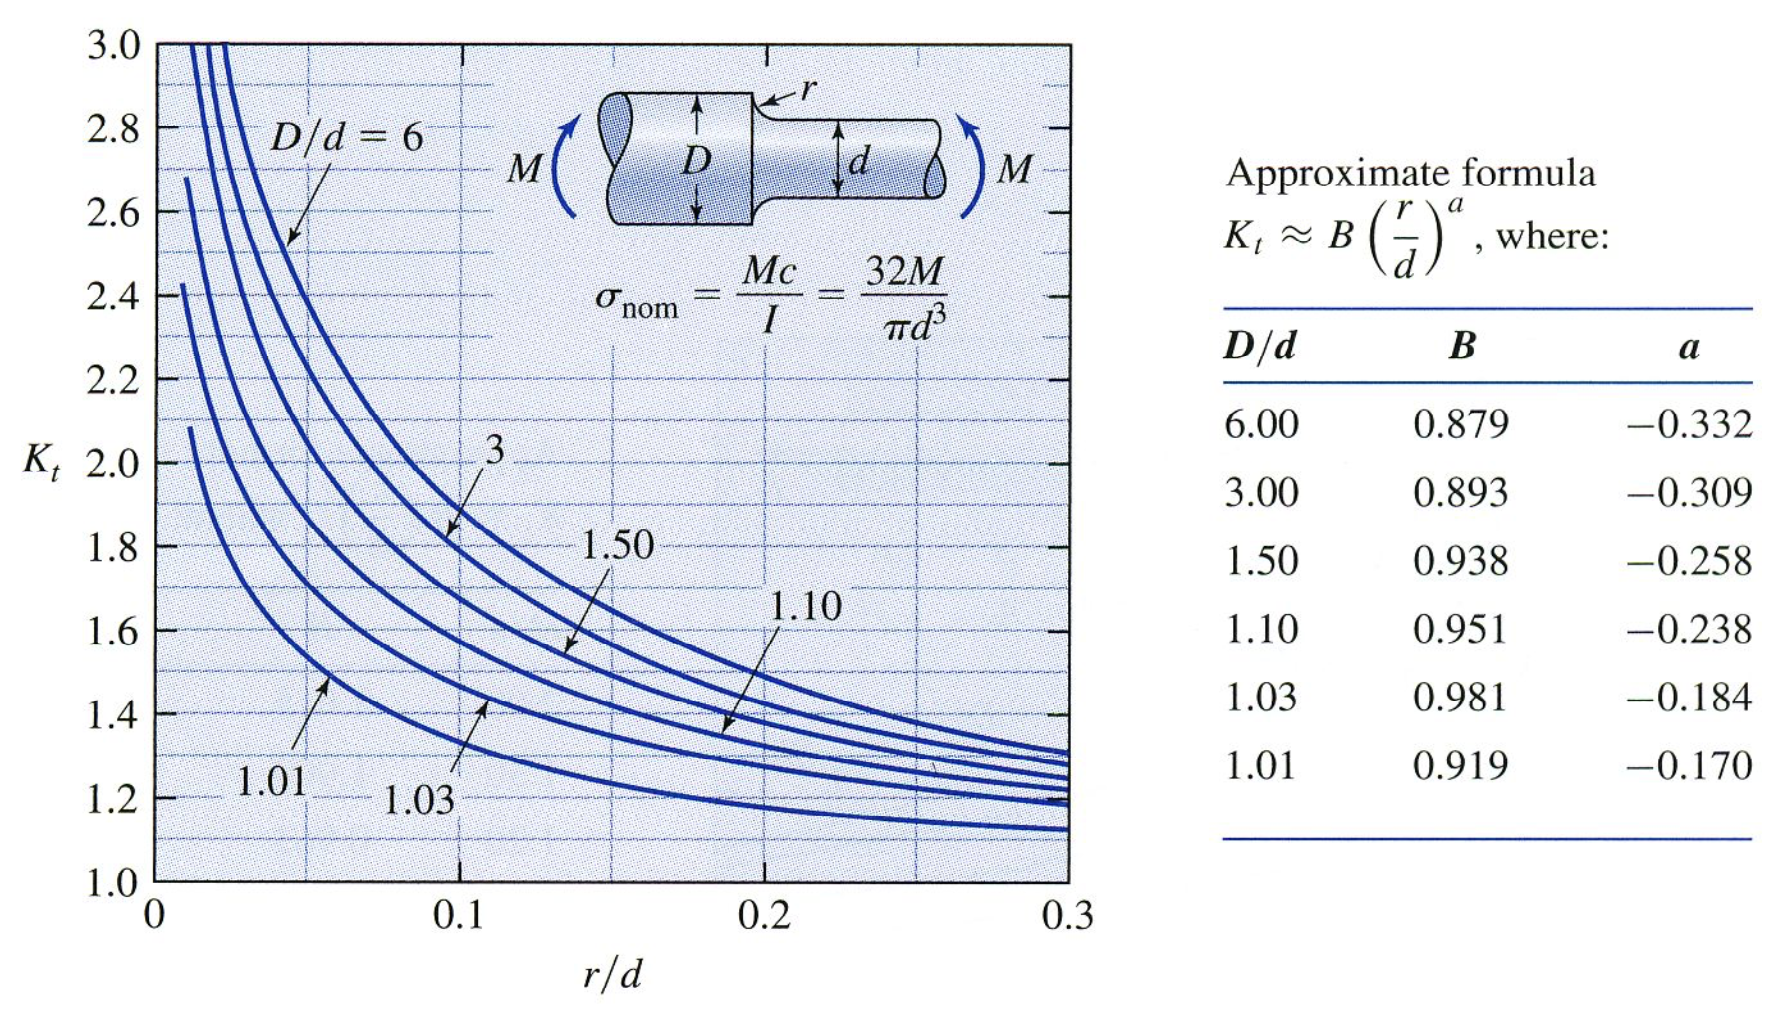
\includegraphics[width=0.45\textwidth]{05_design_factor/fillet-bending.png}
    }
    \hfill
    \subfloat[Shaft under torsion]{
        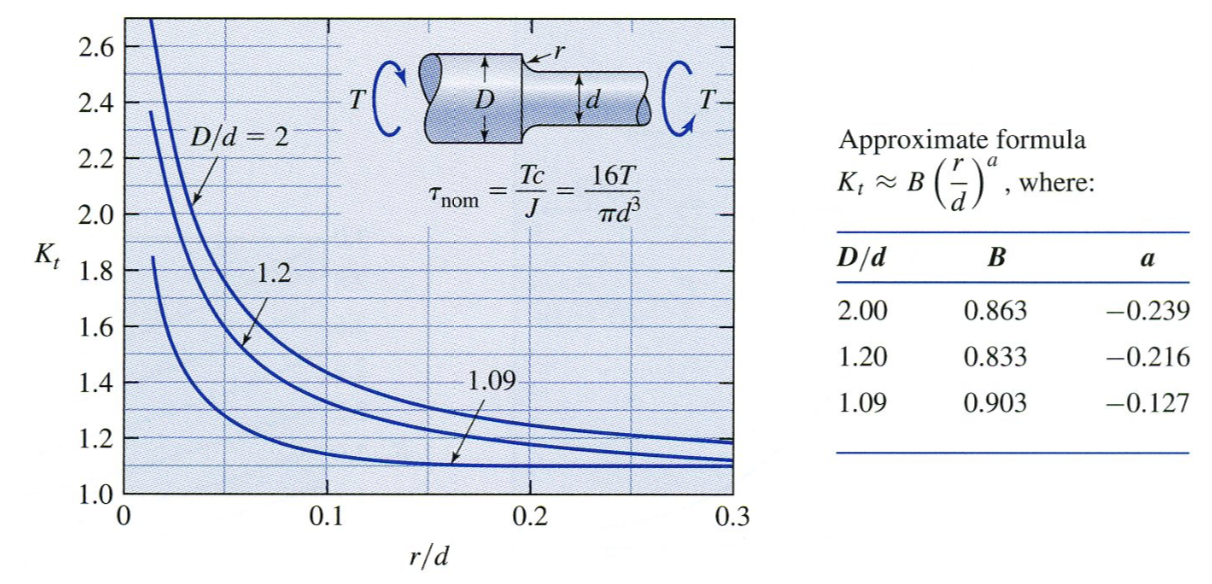
\includegraphics[width=0.45\textwidth]{05_design_factor/fillet-torsion.png}
    }
    \hfill
    
    \vspace{1em}
    \caption{Fillet stress concentration factors for shafts}\label{fig-stress-fillet}
\end{figure*}

\begin{figure*}[t]
    
    \hfill
    \subfloat[Shaft under bending]{
        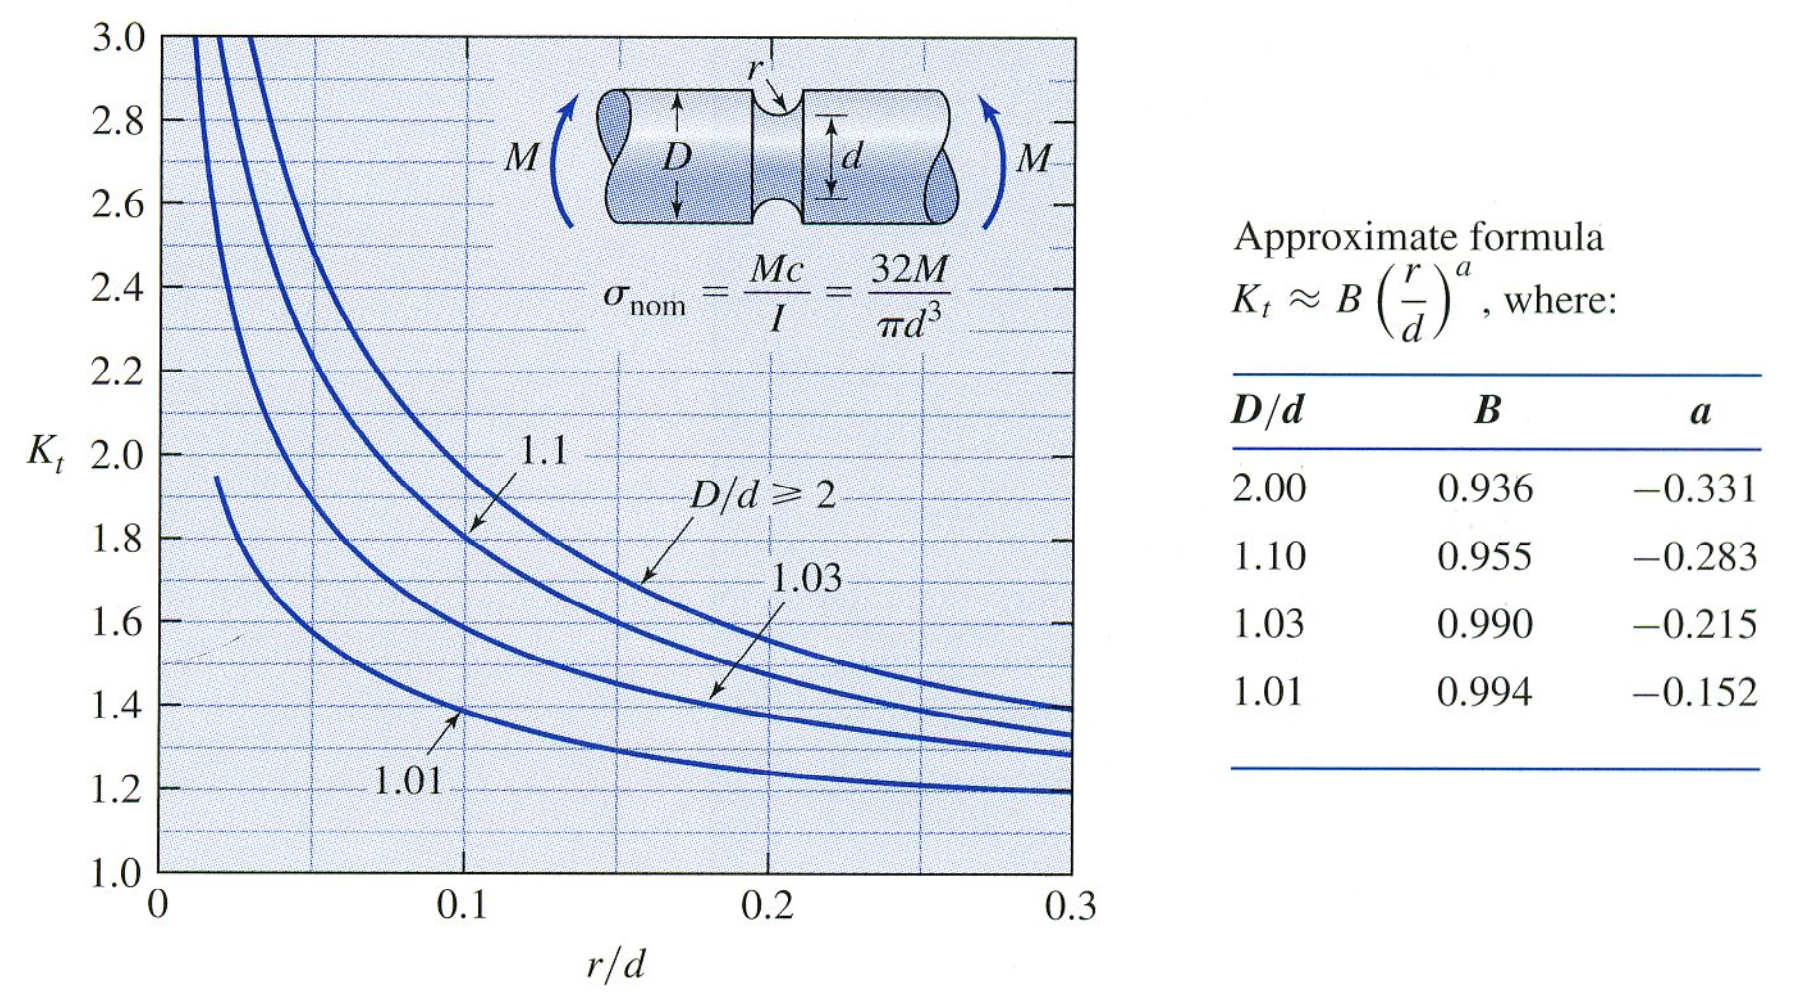
\includegraphics[width=0.45\textwidth]{05_design_factor/circlip-groove-bending.png}
    }
    \hfill
    \subfloat[Shaft under torsion]{
        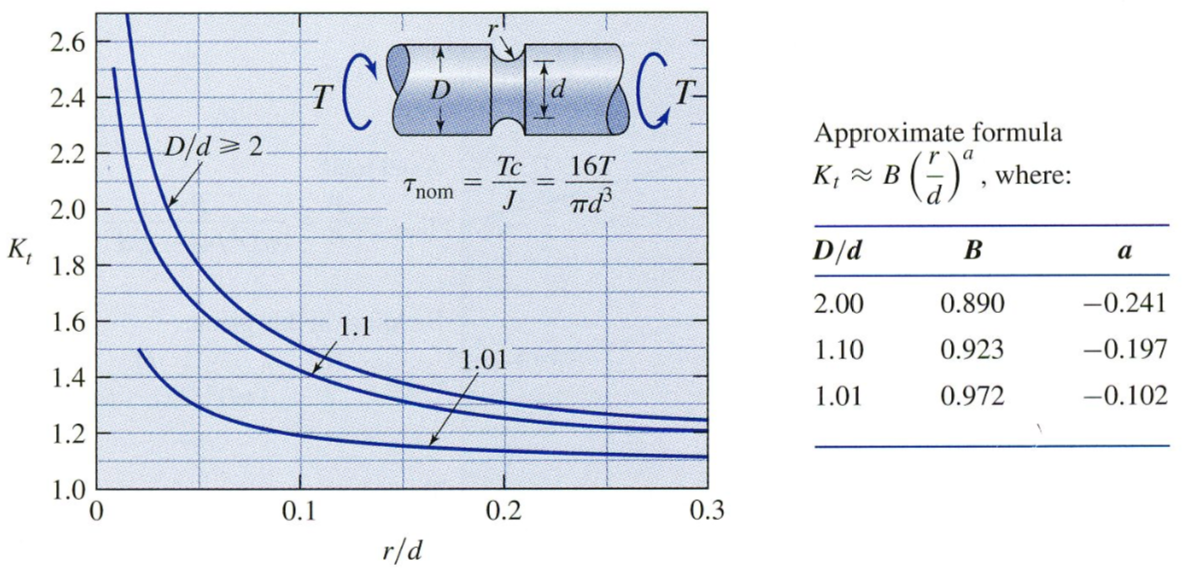
\includegraphics[width=0.45\textwidth]{05_design_factor/circlip-groove-torsion.png}
    }
    \hfill
    
    \vspace{1em}
    \caption{Circlip stress concentration factors for shafts}\label{fig-stress-circlip}
\end{figure*}



\clearpage
\section{Comparing Stress and Allowable Stress}

\newthought{now armed with the calculations} for the shaft stresses and design factor, you will need to select nodes along the shaft that you feel may be critical to its operation. This is for you to decide and to discuss within your reports.

With the nodes selected, you can start to populate the excel spreadsheet that is provided. Placing the calculations within the cells enables you to quickly perform iterations of the shafts design and clearly articulate the changes to the shafts geometry. You will be submitting the final spreadsheet so we can review your calculations within the cells. Please do not alter the format of the spreadsheet. 

\begin{table}[h!]
  \caption{Spreadsheet stress model}
  \centering
  \small
  \begin{tabular}{l | c | c c c}
    \toprule
      & Node No. & 1 & 2 & 3\\
    Node Details & Units & \\
    \midrule
    Diameter \\
    Area \\
    Second Moment of Area \\
    Second Polar Moment of Area \\
    \midrule
    Forces \\
    \midrule
    Vertical \\
    Horizontal \\
    Resultant \\
    Resultant Angle \\
    \midrule
    Bending \\
    \midrule
    Vertical \\
    Horizontal \\
    Resultant \\
    Torque \\
    \midrule
    Stresses \\
    \midrule
    Direct Stress \\
    Bending Stress \\
    Torsional Stress \\
    \midrule
    Principal Stresses \\
    \midrule
    Principal Stress 1 (+) \\
    Principal Stress 2 (-) \\
    Shear Stress \\
    \midrule
    Safety Factors \\
    \midrule
    a \\
    b \\
    c \\
    d \\
    k \\
    Nu \\
    \midrule
    UTS \\
    Allowable Stress \\
    \bottomrule
  \end{tabular}
\end{table}




\clearpage
\section{Transmission Selection}

As part of your design, you will need to select the type of transmission and subsequent specification of your chosen transmission. You will need to do some research on the types of transmission to be able to present a reasoned argument for your selection. This will be followed by the steps taken to select an initial specification of transmission. In this document, we will take your through the selection of a chain transmission. For other transmission types, you will have to look up the relevant guides and processes. Do not let this put you off though as the steps are fairly similar.

\subsection{Transmission Types}

\begin{framed}
    \vspace{1cm}
    \begin{center}
        \Large
        -- Own Research \& Lectures --
    \end{center}
    \vspace{1cm}
\end{framed}

\subsection{Selecting a Chain Drive}

The following selection of a chain drive uses Renold's Chain Guide\footnote{Acknowledgements to the Renold Chain Guide}. Other chain companies will have similar processes and it is important to follow the appropriate companies' process when selecting your transmission.

\subsubsection{Features \& Considerations}

An\marginnote{Centre Distance}  incorrect centre distance leads to a higher wear rate and slack chain, which introduces further inefficiencies into the system. % Centre distances that are smaller than nominal can be attained through the use of a chain tensioner.

When\marginnote{polygonal action} the driving sprocket of a chain drive runs at constant speed, the speed of the chain itself is not constant but is subject to periodic fluctuations. This fluctuation, which is caused by the fact that the chain when wrapped on a sprocket forms a polygon rather than a circle, is known as polygonal action~\cite{mahalingam1958}.

One effect of polygonal action is to produce a periodic variation in the velocity ratio of the drive, and if the frequency of this variation coincides with a resonant frequency of the system, large stresses may occur. At high chain speeds the effects of impact are very complex; each impact sets up a train of travelling waves which, after reflection at the sprockets, combine with the next train and so on.

\cref{fig-cyclic-speed-variation} highlights that polygonal actions' effect increases considerably as one decreases the no.\ of sprocket teeth below 19. Hence, Renold recommends that sprockets should have a minimum of 19 teeth to avoid the effect of polygonal action. If lower teeth are required, then an additional factor is applied when selecting a chain, which reduces the maximum rated speed of the chain.

\begin{marginfigure}
    \centering
    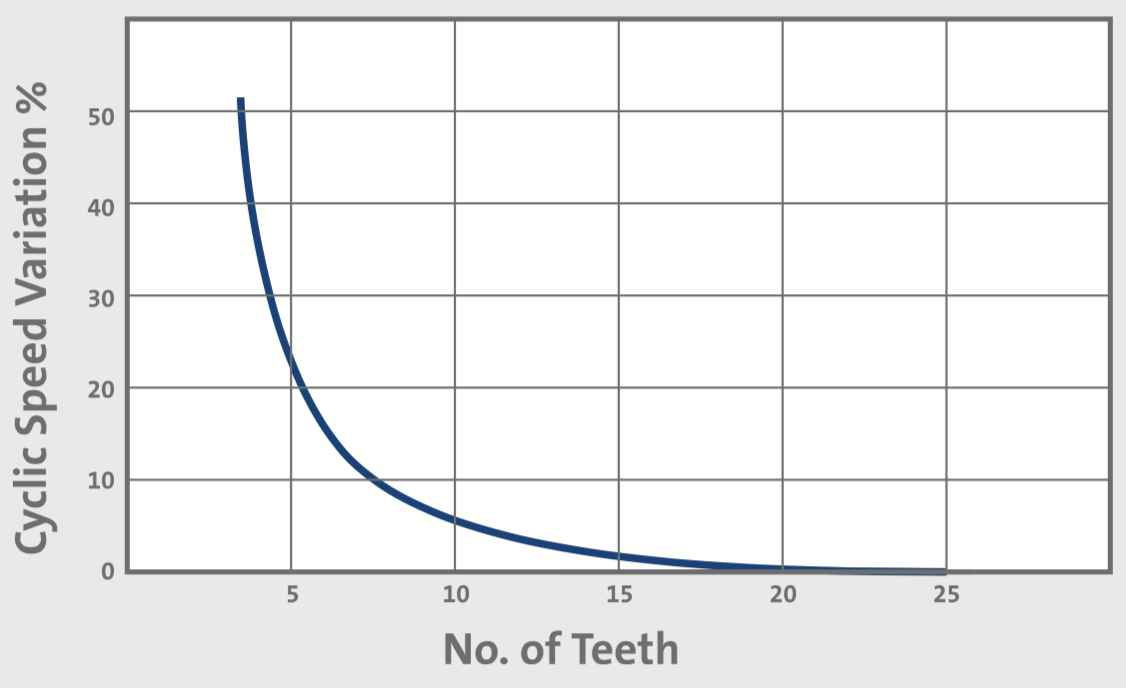
\includegraphics[width=\textwidth]{07_transmission_selection/polygonal-action.png}
    \caption[Cyclic speed variation due to polygonal action]{Cyclic speed variation due to polygonal action~\citep[p.24]{renoldchain}}
    \label{fig-cyclic-speed-variation}
\end{marginfigure}

It\marginnote{cranked link} is always best practice and desirable to have a chain with an even number of links. However, when there is a case that requires an odd linked chain, cranked links are used to form the chain loop. \cref{fig-cranked-link} shows an example of a cranked link within a chain. The link has a natural kink in the profile to allow it to connect to the next link in the chain. This inherently places additional stress concentrations within the component and thus, is not recommended for high load and/or speed chain drives.


\begin{marginfigure}
    \centering
    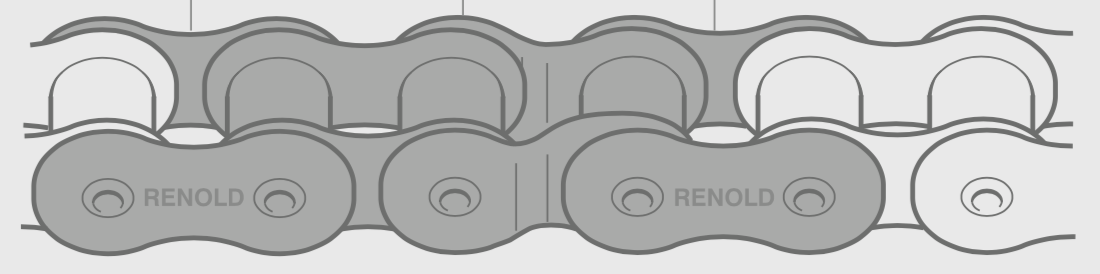
\includegraphics[width=\textwidth]{07_transmission_selection/cranked-link.png}
    \caption[Cranked link]{Cranked link~\citep[p.11]{renoldchain}}
    \label{fig-cranked-link}
\end{marginfigure}

\subsubsection{Selection Process}

The selection process for a Renold chain is as follows. The prerequisites for the process is that you know the torque and sprocket speeds that you wish to run at.

The\marginnote{Selection Power (\(P_s\))} selection power is calculated by multiplying the power you wish to transmit (\(P_s\)) by two safety factors \(f_1\) and \(f_2\).

\begin{equation}
  P_s = f_1f_2P_t
\end{equation}

\noindent Where:

\begin{description}
  \item[\(f_1\)] Safety factor depending on your operation and can be found using chart 2 on p.28 of the Renold catalogue
  \item[\(f_2\)] Adjustment factor is your are using the non-recommended number of driving sprocket teeth. \(f_2=\frac{19}{\text{No. of teeth on driving}}\)
\end{description}

With\marginnote{Selecting a Suitable Chain Pitch} the selection power determined and the driver sprocket speed known, one can determine the chain pitch using \cref{fig-chain-pitch}. These rating charts have been created from years of empirical testing and theoretical modelling by the chain companies, and dictate the safe operating windows for their selection of chains.

\begin{figure}[h!]
    \centering
    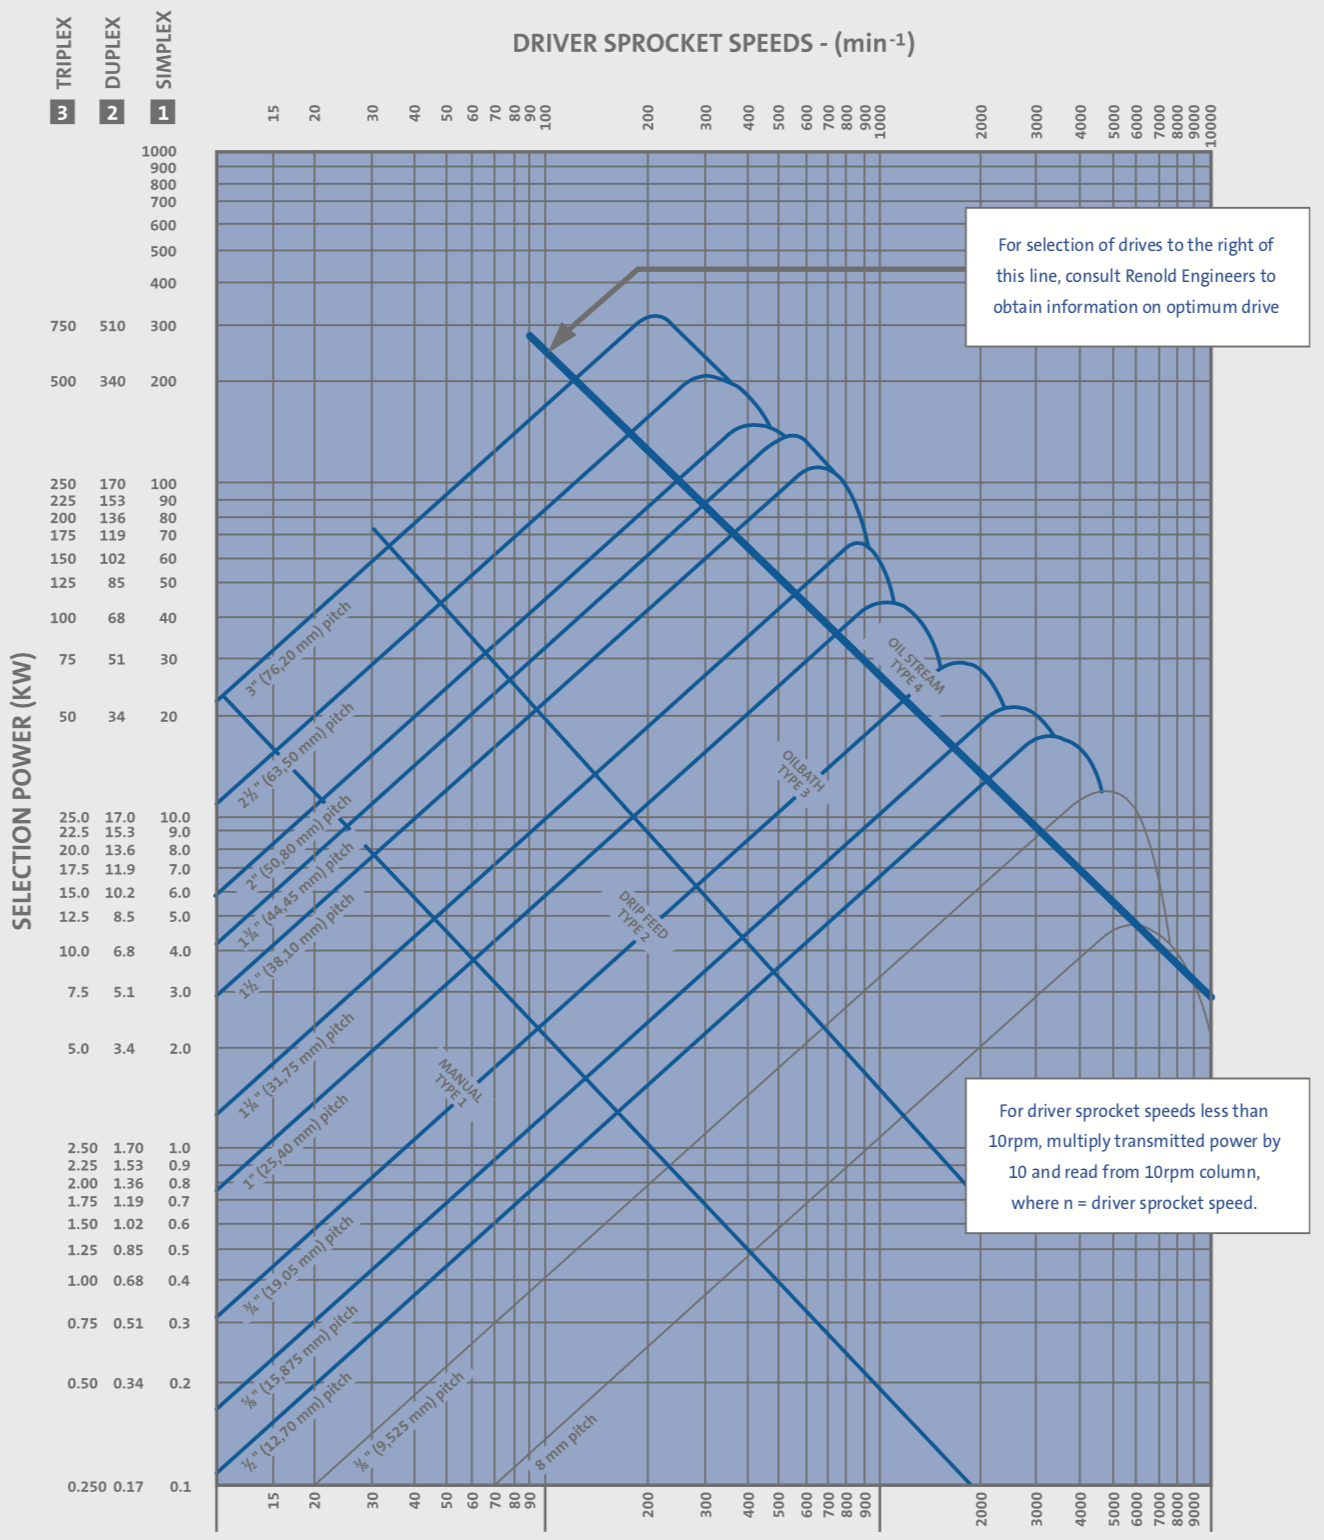
\includegraphics[width=0.9\textwidth]{07_transmission_selection/chain-pitch.png}
    \caption[Chain pitch selection chart]{Chain pitch selection chart~\citep[p.31]{renoldchain}}
    \label{fig-chain-pitch}
\end{figure}

After\marginnote{Select Chain and Sprockets} selecting the chain pitch, you can go through the catalogue to find the drive and driven sprockets that will give you the required (or as near as possible) ratio for your design.

Having\marginnote{Chain Links and Centre Distance} the chain pitch and sprockets selected, the centre distance

\begin{equation}
    L = \frac{Z_1+Z_2}{2}+\frac{2C_1}{P}+\frac{P{\left(\frac{Z_2-Z_1}{2\pi}\right)}^2}{C_1}
\end{equation}

\noindent{} Where:

\begin{description}
    \item[\(Z_1\)] Number of driving teeth
    \item[\(Z_2\)] Number of driven teeth
    \item[\(C_1\)] Approximate desired centre distance
    \item[\(P\)] Chain pitch
    \item[\(L\)] Number of chain links
\end{description}

Once calculated, you then round to the nearest even integer and use this to calculate your centre distance \(C\).

\begin{equation}
    C=\frac{P}{8}
    \left[
    2L-Z_2-Z_1 
    +
    \sqrt{ 
    {\left(2L-Z_2-z_1\right)}^2 - \left(\frac{\pi}{3.88}\left(Z_2-Z_1\right)^2\right)
    }
    \right]
\end{equation}

\subsubsection{Chain Example}

Select a chain and sprocket to transmit \SI{2}{\kilo\watt} of power at \SI{20}{rpm}. A ratio of 1:2 is required, driven by an electric motor with moderate shocks expected from the load. Space is highly limited.

Using\marginnote{determining \(f_1\) and \(f_2\)} Chart 2 on p.28 of the Renold catalogue, we identify that \(f_1=1.4\) for our context and we will also use the recommended number of teeth on the driving sprocket (19), which makes \(f_2=1\). Therefore, the selection power \(P_s\) becomes:

\begin{equation}
    P_s = f_1f_2P_t = 2\si{\kilo\watt}\times1.4\times1=2.8\si{\kilo\watt}
\end{equation}

Using\marginnote{chain pitch} \cref{fig-chain-pitch}, we can find the chain pitches that are suitable for our application. The potential pitches are:

\begin{itemize}
    \item \SI{38.10}{\milli\metre} simplex
    \item \SI{31.75}{\milli\metre} duplex
    \item \SI{25.40}{\milli\metre} triplex
\end{itemize}

For\marginnote{chain and sprocket selection} this example, we will select the triplex as our requirement is to have a compact solution. Now it is just a case of looking in the tables to find a sprocket set (Renolds, p.75) that will provide us with a ratio that provides us with the closest match in terms of our desired ratio, and a triplex chain (Renolds, p.25).

\begin{description}
    \item[Chain] 12B-3
    \item[Driving Sprocket] 16B1/19T
    \item[Driven Sprocket] 16B1/38T
\end{description}

Now\marginnote{chain links} we have the sprockets and chain selected, it is then a simple case of using their specifications to determine the number of links:

\begin{equation}
    L = 
    \frac{19+38}{2}
    +
    \frac{2\times571.5}{19.05}+\frac{19.05{\left(\frac{38-19}{2\pi}\right)}^2}{571.5} = 88.6
\end{equation}

Rounding this up to the nearest even integer gives us \(L=90\).

The\marginnote{centre distance} final calculation is to determine the centre distance:

% https://www.sharelatex.com/learn/Aligning_equations_with_amsmath
\begin{equation}
\begin{split}
    C & = \frac{19.05}{8}
    \left[
    2(90)-38-19 
    +
    \sqrt{ 
    {\left(2(90)-38-19\right)}^2 - \left(\frac{\pi}{3.88}\left(38-19\right)^2\right)
    }
    \right] 
    \\ & = \SI{583}{\milli\metre}
\end{split}
\end{equation}

\subsection{Selecting a vee-belt or tooth belt}

\begin{framed}
    \vspace{1cm}
    \begin{center}
        \Large
        -- Own Research \& Lectures --
    \end{center}
    \vspace{1cm}
\end{framed}



\clearpage
\section{Bearing Selection}

This section details the process in selecting bearings from the SKF catalogue. However, it is up to you to do your own research and attend the lectures to understand and determine the most appropriate bearings for your design problem.

\subsection{Bearing Types and Locating Bearings}

\begin{framed}
    \vspace{1cm}
    \begin{center}
        \Large
        -- Own Research \& Lectures --
    \end{center}
    \vspace{1cm}
\end{framed}

%\marginnote{Deep-Groove Ball \\ 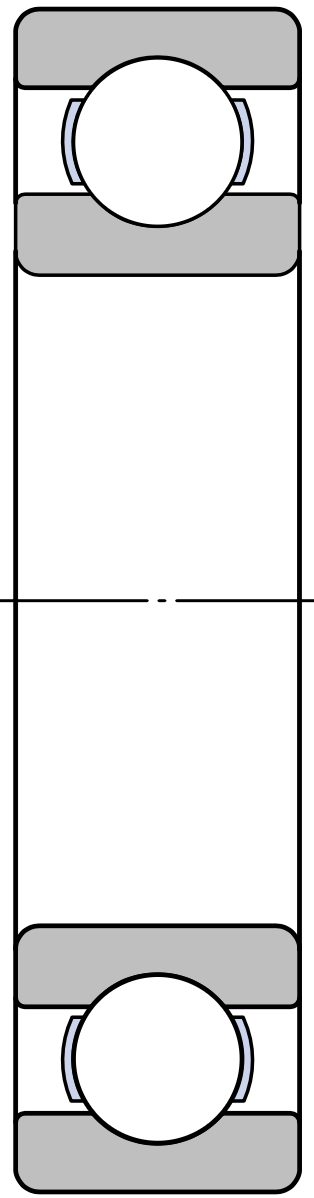
\includegraphics[width=0.06\textwidth]{single-deep-groove-ball-bearing.png}}

%\vspace{3cm}

%\marginnote{Angular Contact Bearing \\ 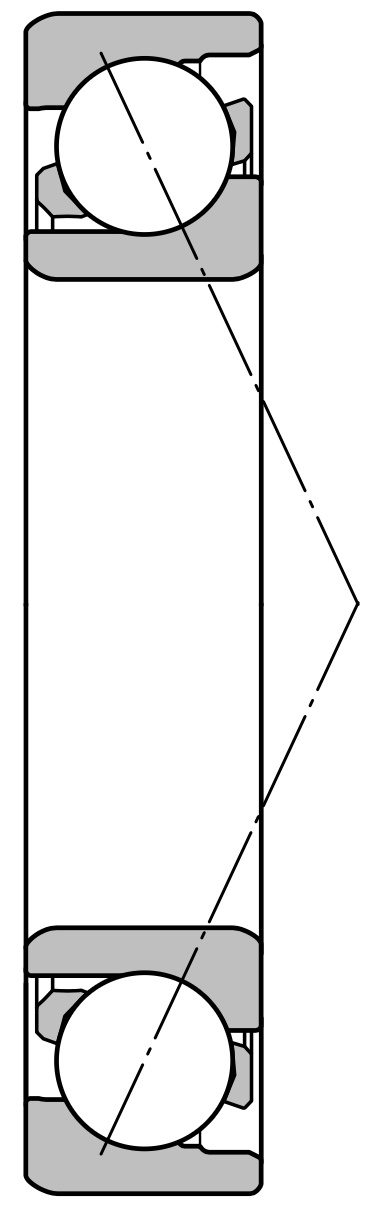
\includegraphics[width=0.07\textwidth]{angular-contact-bearing.png}}

%\vspace{3cm}

%\marginnote{Taper Roller \\ 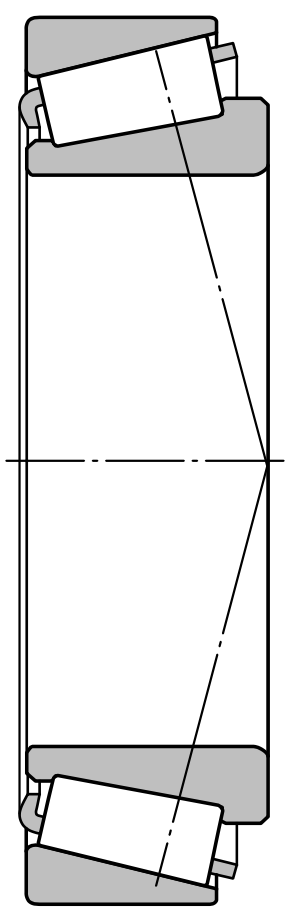
\includegraphics[width=0.07\textwidth]{taper-bearing.png}}

%\vspace{3cm}

%\marginnote{Cylindrical Roller \\ 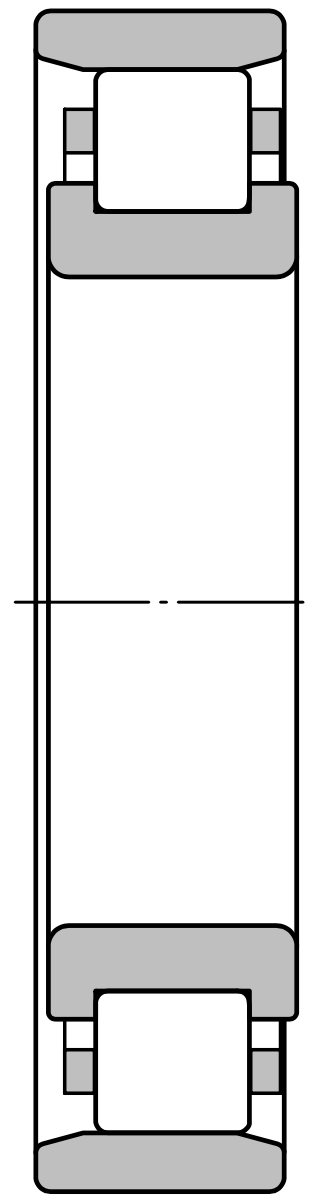
\includegraphics[width=0.07\textwidth]{cylindrical-roller-bearing.png}}

%\vspace{3cm}

%\marginnote{Y-Bearing \\ 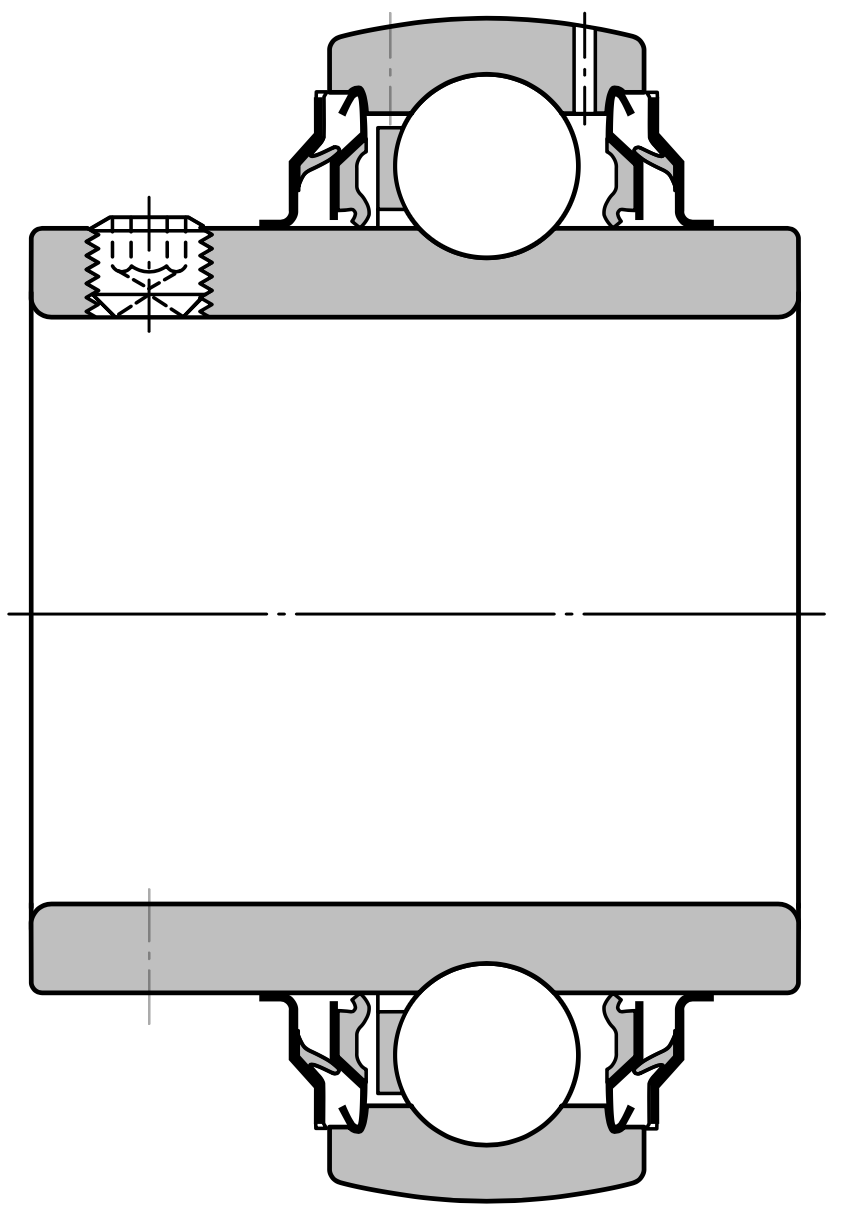
\includegraphics[width=0.2\textwidth]{y-bearing.png}}

%\vspace{3cm}

%\subsection{Locating Bearings}

%\begin{framed}
%  \vspace{2cm}
%    \begin{center}
%      {\fontsize{50}{60}\selectfont \faQuestion{}}\\
%      Research Required
%    \end{center}
%  \vspace{2cm}
%\end{framed}

%\marginnote{\it float}

%\marginnote{\it stepped shaft}

%\marginnote{\it fillet radius}

%\marginnote{\it spacer}

%\marginnote{\it undercut}

%\marginnote{\it pre-load}

\subsection{Bearing Calculations} 

Once you have decided upon the bearing arrangement for your shaft, we can use SKF's bearing selection process to determine the size of bearing that is required. Manufacturers often provide a selection process for their bearings, which they have developed over years of experience in designing and manufacturing their products. The SKF process requires us to determines the basic dynamic \(C\) and static \(C_0\) load ratings that we require for our bearings, which are in accordance of ISO 281:2007 and ISO 76:2006, respectively.


Lets\marginnote{Basic Static Load Rating (\(C_0\))}  start with calculating the basic static load rating for a bearing. This can be calculated using Equation~(\ref{equ-basic-load-rating}) and is where the equivalent static load \(P_0\) is multiplied by a safety factor \(S_0\).

\begin{equation}
    C_0 = P_0 S_0
    \label{equ-basic-load-rating}
\end{equation}

Thus, we need to know both \(P_0\) and \(S_0\).

The\marginnote{Equivalent Static Load (\(P_0\))} calculation for \(P_0\) is dependent upon the type of bearing you're looking to selecting. In the case of a deep-groove ball bearing, \(P_0\) is calculated by:

\begin{equation}
    \text{Calculate } P_0 = 0.6F_r+0.5F_a \text{ then if, } P_0 \le F_r \text{ we set, }P_0 = F_r
\end{equation}

This\marginnote{Safety Factor (\(S_0\))} is then multiplied by the Safety Factor (\(S_0\)), which is selected based on the shafts operating condition.

\begin{itemize}
    \item 0.5 for smooth and shock free
    \item 1.0 for normal
    \item 1.5 for shock and vibration
\end{itemize}

Now\marginnote{Basic Dynamic Load Rating (\(C\))}  we have calculated \(C_0\), we can move onto the basic dynamic load raring (\(C\)), which is calculated through the re-arrangement of the following equation:

\begin{equation}
    L_{10} = \left(\frac{C}{P}\right)^p
    \label{equ-bearing-life}
\end{equation}

\noindent{} Where:

\begin{description}
    \item[\(L_{10}\)] Is the number of revolutions at constant speed that 90\% of bearings tested will complete or exceed before the first evidence of failure develops. This is usually standardised to 1,000,000 cycles in accordance with ISO 281:2007.
    \item[\(C\)] basic dynamic loading rating (\si{\kilo\newton})
    \item[\(P\)] equivalent dynamic bearing load (\si{\kilo\newton})
    \item[\(p\)] bearing factor
    \begin{itemize}
        \item Ball Bearing, \(p=3\)
        \item Roller Bearing, \(p=\frac{10}{3}\)
    \end{itemize}
\end{description}

Thus, to calculate \(C\), we need to know both \(L_{10}\) and \(P\).

To\marginnote{life rating (\(L_{10}\))} determine the life rating (in cycles),

\begin{equation}
    L_{10} = \text{Hours of Operation} \times \text{rpm} \times 60
\end{equation}

With\marginnote{Equivalent Dynamic Bearing Load (\(P\))} \(L_{10}\) now known, we can focus our attention onto \(P\). The calculation for \(P\) is dependent upon the type of bearing you're looking to selecting. In the case of a deep-groove ball bearing (SKF p.316).

\begin{equation}
    P = XF_r + YF_a
\end{equation}

To determine the coefficients \(X\) and \(Y\), we need to find the calculation factors \(f_0\) and \(e\).

From the catalogue, \(f_0\) is calculated using:

\begin{equation}
    f_0 = \frac{F_a}{C_0}
\end{equation}

And \(e\) can be found using the look-up table on page XX in the catalogue. In this case, \(e=0.22\). With these values, we can then decide on, which equivalent dynamic bearing load calculation we require (SKF p.316). One example is:

\begin{equation}
    \text{if, }\frac{F_a}{F_e}\le e \Rightarrow P=F_r \text{ else, } \frac{F_a}{F_e}\ge e \Rightarrow P=XF_r+YF_a
\end{equation}

Once we have \(P\), we can calculate \(C\) be re-arranging the life rating equation (\cref{equ-bearing-life}). 

\begin{equation}
    \sqrt[p]{L_{10}}\times P = C
\end{equation} 

With\marginnote{Finding a Bearing} \(C_0\) and \(C\) calculated, it is then just a case of looking through the bearing tables and finding a bearing that meets these criteria.

\subsection{Example: Deep Groove Ball Bearing Selection}

A deep groove ball bearing is needed to support a \SI{15}{\kilo\newton} radial and \SI{3}{\kilo\newton} axial loading rotating at \SI{30}{rpm}, on a shaft of \SI{30}{\milli\metre} diameter. The bearing will operate in a smooth-running environment without shock loading, and must be reliable for \SI{5000}{\hour} of operation.

From this description, we can quickly ascertain that:

\begin{itemize}
    \item Deep Groove Ball. Therefore, \(p=3\)
    \item Running speed \(\ge \SI{10}{rpm}\). Therefore, the dynamic load rating is required \(P=XF_r+YF_a\)
    \item Smooth running, vibration free and low shock loading. Therefore, the safety factor \(S_0\) is 1.
    \item \(L_{10} = 5000 \times 60 \times 30 = 9,000,000\) cycles 
\end{itemize}

\marginnote{Equivalent Static Load (\(P_0\))} Using the SKF catalogue, the equivalent static bearing load is given by:

\begin{equation}
    P_0 = 0.6F_r+0.5F_a \text{ then if, } P_0 \le F_r \text{ we set, }P_0 = F_r
\end{equation}

\noindent{} Hence, for this case, \(P_0\) is:

\begin{equation}
    P_0=0.6F_r+0.5F_a = 0.6\times\SI{15}{\kilo\newton} + 0.5\times\SI{3}{\kilo\newton} = \SI{10.5}{\kilo\newton}
\end{equation}

\noindent{} As \(P_0 \le F_r \), we set \(P_0 = F_r = 15\si{\kilo\newton} \).

Now\marginnote{Basic Static Load Rating (\(C_0\))} we can calculate our static load rating \(C_0\) using:

\begin{equation}
    C_0=P_0S_0
\end{equation}

\noindent{} And for our case, \(C_0\) becomes:

\begin{equation}
    C_0= \SI{15}{\kilo\newton} \times 1 = \SI{15}{\kilo\newton}
\end{equation}


Having\marginnote{Equivalent Dynamic Load (\(P\))} calculated \(C_0\), we can move onto calculating the equivalent dynamic load \(P\) so that we can attain the basic dynamic load rating \(C\):

\begin{equation}
    P = XF_r + YF_a
\end{equation}

To determine the coefficients \(X\) and \(Y\), we need to find the calculation factors \(f_0\) and \(e\).

From the catalogue, \(f_0\) is calculated using:

\begin{equation}
    f_0 = \frac{F_a}{C_0} = \frac{3\si{\kilo\newton}}{15\si{\kilo\newton}} = 0.2
\end{equation}

And \(e\) can be found using the look-up table on p.315 in the catalogue. In this case, \(e=0.22\). With these values, we can then decide on, which equivalent dynamic bearing load calculation we require (SKF p.316). 

\begin{equation}
    \text{if, }\frac{F_a}{F_r}\le e \Rightarrow P=F_r \text{ else, } \frac{F_a}{F_r}\ge e \Rightarrow P=XF_r+YF_a
\end{equation}

Therefore, in our case:

\begin{equation}
    \frac{F_a}{F_r}=\frac{3\si{\kilo\newton}}{15\si{\kilo\newton}}=0.2
\end{equation}

\noindent{} and this value is \(\le e\). Thus, 

\begin{equation}
    P=F_r=15\si{\kilo\newton}
\end{equation}

Now\marginnote{Equivalent Dynamic Load Rating (\(C\))} we have all the information we need to determine the equivalent dynamic load rating \(C\) by re-arranging the life rating equation (Equation~\ref{equ-bearing-life}). 

\begin{equation}
    \sqrt[p]{L_{10}}\times P = C = \SI{31.2}{\kilo\newton}
\end{equation}

Now looking through the available bearings in the catalogue and knowing we have to fit onto a \SI{30}{\milli\metre} shaft, two bearings are potentially suitable:

\begin{itemize}
    \item 6306 ETN9
    \item 6406
\end{itemize}

Looking into more detail of the designations of the bearings reveals that ETN9 means that the bearing is reinforced. This is likely to be an over-specification for our application. Therefore, we shall select 6406.

%\subsection{Bearing Selection -- Roller Bearing Example}

%A locating roller bearing is needed to support a 60\si{\kilo\newton} radial and 25\si{\kilo\newton} axial loading rotating at 100\si{rpm}, on a shaft of 75\si{\milli\metre} diameter. The bearing will operate in a normal environment, and must be reliable for 11,000\si{\hour} of operation.

%\begin{itemize}
%  \item Roller. Therefore, \(p=\frac{10}{3}\)
%  \item Running speed \(\ge 10\si{rpm}\). Therefore, the dynamic load rating is required.
%  \item Normal running environment. Therefore, the safety factor \(S_0\) is 1.
%  \item \(L_{10} = 11,000 \times 60 \times 100 = 66,000,000\) cycles 
%\end{itemize}

%\marginnote{Basic Static Load Rating} [TO DO]

%\marginnote{Equivalent Dynamic Load \(P\)} Looking through the SKF catalogue, we identify the equation for \(P\) for locating bearings (p.594).

%\begin{equation}
%\text{If } \frac{F_a}{F_r} \leq e \text{ then } P=F_r \text{ else } P=0.92F_r+YF_a
%\end{equation}

%\begin{equation}
%  \frac{F_a}{F_r}=\frac{25\si{\kilo\newton}}{60\si{\kilo\newton}} = 0.417 > e
%\end{equation}

%To determine \(Y\), we look up the value in the respective SKF table (p.593). In this case, \(Y=0.6\). Thus, \(P\) becomes:

%\begin{equation}
%  P=0.92F_r+0.6F_a=70.2\si{\kilo\newton}
%\end{equation} 

%\marginnote{Basic Dynamic Load Rating \(C\)} Now we have \(P\), we can calculate the basic dynamic load rating \(C\).

%\begin{equation}
%  \sqrt[p]{L_{10}}\times P = C = \sqrt[\frac{10}{3}]{66,0000,000}\times 70,200=246\si{\kilo\newton}
%\end{equation}


%Looking through the SKF tables, we can find a range of suitable bearings with NUP designated bearings able to take axial loads. Focusing on these bearings, two options are available to us:

%\begin{itemize}
%  \item NUP 135 ECP
%  \item NUP 2135 ECP
%\end{itemize}


\clearpage
% http://www.thecartech.com/subjects/machine_elements_design/keys_and_Splines.htm

\section{Shaft Fixtures and Fittings}

This section provides descriptions of a few fixtures and methods of fitting components to a shaft. You may need to use this in your exercise as well as performing your own research on other techniques that might be suitable.

\subsection{Spline}

\begin{marginfigure}
    \centering
    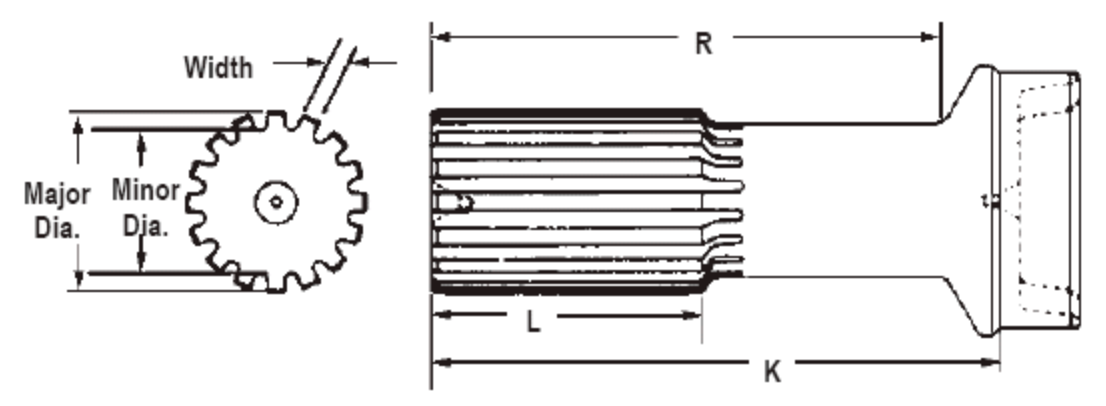
\includegraphics[width=\textwidth]{09_fixtures_and_fittings/spline-shaft.png}
    \caption{Spline shaft}
\end{marginfigure}
Splines are ridges or teeth on a drive shaft that mesh with grooves in a mating piece. This enables the transfer of high torque loads, whilst maintaining angular correspondence. There are a number of different types including:

\begin{itemize}
    \item Parallel key spline
    \item Involute spline
    \item Crowned splines
    \item Serrations
    \item Helical splines
    \item Ball splines
\end{itemize}

Here are some calculations often used for splines\sidenote{\url{http://www.thecartech.com/subjects/machine_elements_design/keys_and_Splines.htm}}.

The first is the calculation of the Torque capacity for a spline and this is given by:\marginnote{Torque Capacity of Spline}

\begin{equation}
    T=pAr_m
\end{equation}

\noindent where:

\begin{description}
    \item[\( p \)] Permissibale pressure on the splines (\(<7\si{\mega\pascal}\), if relative axial motion)
    \item[\(A\)] Total load area of splines (\(0.5(D-d)Ln\), \si{\metre^2})
    \item[\(D\)] Outer spline shaft diameter (\si{\metre})
    \item[\(d\)] Inner spline shaft diameter (\si{\metre})
    \item[\(L\)] Length of spline (\si{\metre})
    \item[\(n\)] Number of splines
    \item[\(r_m\)] Mean radius (\si{\metre})
\end{description}

The shear that a spline experiences can be calculated as follows:\marginnote{Spline Shear}

\begin{equation}
    \tau = \frac{4T}{Lbn(D+d)}
\end{equation}

where:

\begin{description}
    \item[\( F \)] Force acting on a spline 
    \item[\( b \)] Spline width
    \item[\( n \)] Number of splines
\end{description}


%\marginnote{Spline in Bending}

%\begin{equation}
%  \sigma_b = \frac{3F(D-d)}{b^2Ln}
%\end{equation}

%\marginnote{Pressure on groove supporting surface} 

%\begin{equation}
%  d_{\min} = \sqrt[3]{\frac{16T K_a S_v}{\pi{} \tau K_f}}
%\end{equation}

%where:

%\begin{description}
%  \item[\( d_{\min} \)] Minimal shaft diameter
%  \item[\(T\)] Torque (\si{\newton\metre})
%  \item[\(K_a\)] Application factor
%  \item[\(K_f\)] Fatigue-life factor
%  \item[\(S_v\)] Desired safety
%  \item[\(\tau\)] Allowable shear stress (\si{\pascal})
%\end{description}


\subsection{Taper Lock} 


The Taper Lock bush, also referred to as a Taper bush or Taper Fit bush, is a locking mechanism commonly used in Power Transmission Drives for locating pulleys, sprockets, and couplings to shafts. 
The Taper Lock bush is pre-bored and keyed to match the required shaft and keyway diameters. 
The outside of the bush is tapered to match the component bore that is to be located on the shaft.
\begin{marginfigure}
    \centering
    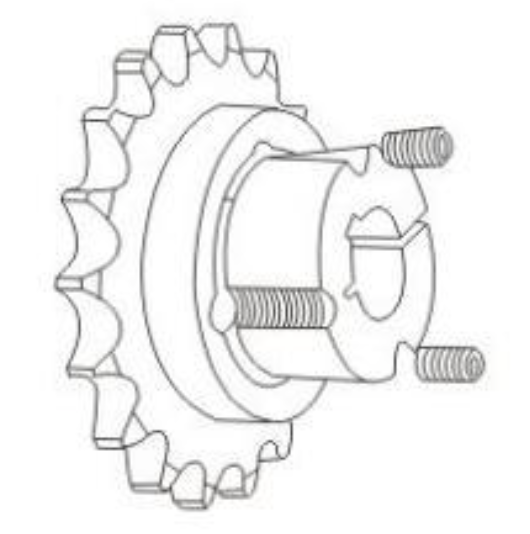
\includegraphics[width=\textwidth]{09_fixtures_and_fittings/taper-lock.png}
    \caption{Taper lock}
\end{marginfigure}

\subsection{Keyway} 

Keyways are a common method of transmitting the torque from the shaft to an attached component such as a sprocket.

\begin{figure}[h!]
    \centering
    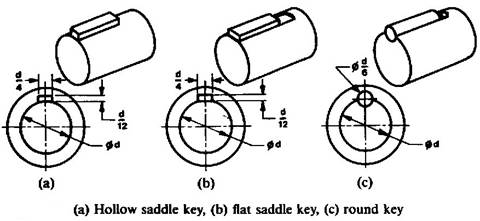
\includegraphics[width=\textwidth]{09_fixtures_and_fittings/keys.jpg}
    \caption{Types of key}
\end{figure}

When\marginnote{Determining the Minimum Key Size} a torque is applied, a key experiences two stress, a shear stress \(\tau\) and compressive stress \(\sigma_c\). These can be calculated as follows:

\marginnote{key shear (\(\tau\))}

\begin{equation}
  \tau = \frac{T}{wLr}
\end{equation}

\noindent{}Where:

\begin{description}
    \item[\(\tau\)] Key shear (\si{\pascal})
    \item[\(T\)] Torque (\si{\newton\metre})
    \item[\(w\)] Key width (\si{\metre})
    \item[\(L\)] Key length (\si{\metre})
    \item[\(r\)] Shaft radius (\si{\metre})
\end{description}

\marginnote{Key Compressive Stress (\(\sigma_c\))}

\begin{equation}
    \sigma_c = \frac{T}{0.5tLr}
\end{equation}

\noindent{}Where:

\begin{description}
    \item[\(\sigma_c\)] Compressive stress (\si{\pascal})
    \item[\(T\)] Torque (\si{\newton\metre})
    \item[\(t\)] Key height (\si{\metre})
    \item[\(L\)] Key length (\si{\metre})
    \item[\(r\)] Shaft radius (\si{\metre})
\end{description}

\marginnote{Standard Key Sizes} Although you can calculate the exact dimensions required for your key, there are standards for key sizes. Therefore, you can select any that meet your minimum requirements.

\begin{figure}[h!]
    \centering
    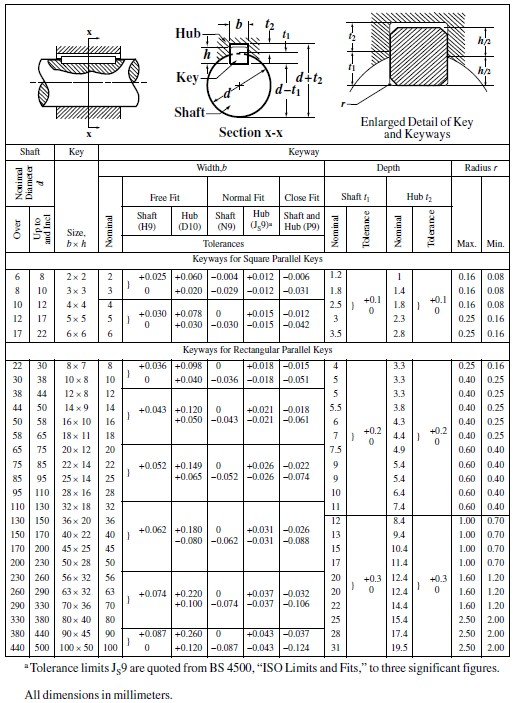
\includegraphics[width=0.8\textwidth]{09_fixtures_and_fittings/key-selection.jpg}
    \caption{An example of a key selection chart}
\end{figure}

\subsection{Circlip}

Circlips are a type of fastener consisting of a semi-flexible metal ring with open ends, which can be snapped into a machined groove on a dowel pin or other part to permit rotation but to prevent lateral movement. 
There are two basic types: internal and external, referring to whether they are fitted into a bore or over a shaft.
Circlips are often used to secure pinned connections.
There are many vendors that can provide circlips and provide information such as the one in \cref{tbl-circlip} to aid in the selection of the appropriate size clip for your needs.

\begin{table}[h!]
    \caption{An example of an external circlip information sheet}\label{tbl-circlip}
    \centering
    \scriptsize
    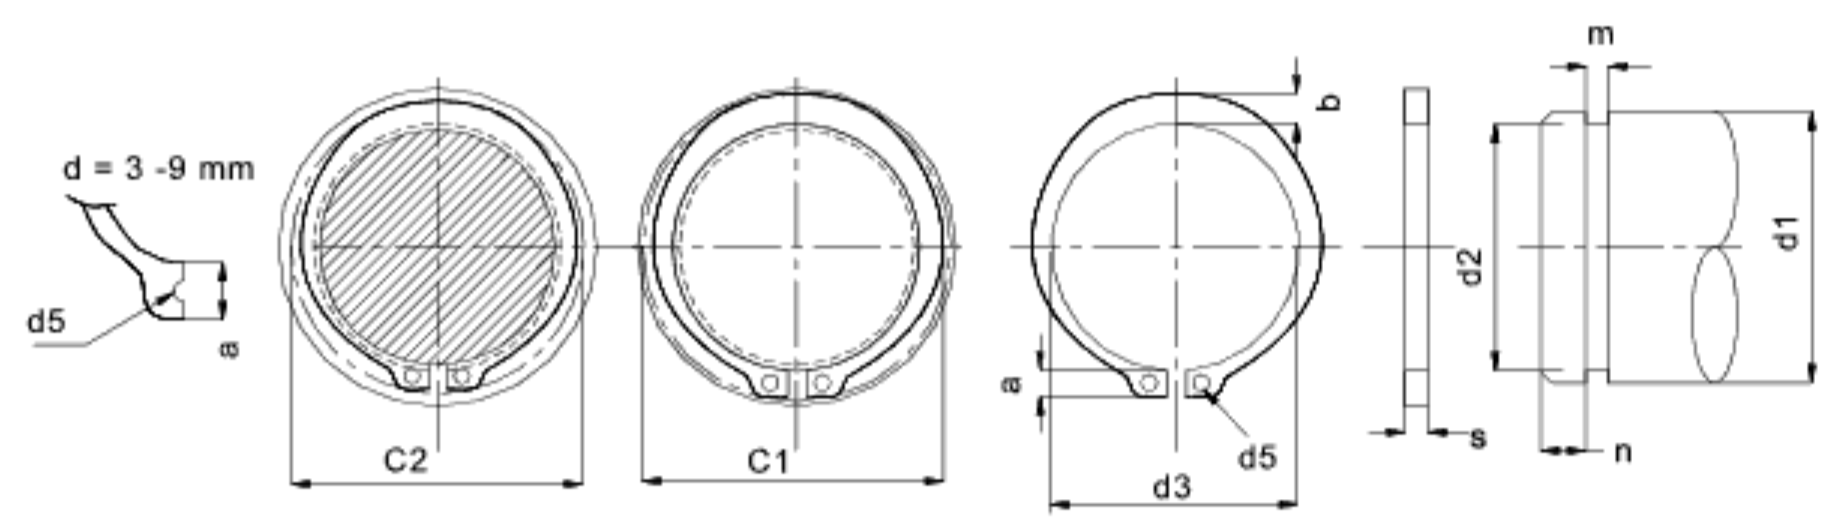
\includegraphics[width=0.8\textwidth]{09_fixtures_and_fittings/circlip-dimensions.png}
    \begin{tabular}{r r r r r r r r r r r r r r r r r}
    \toprule
    \multicolumn{1}{p{0.05\textwidth}}{Nom size (\si{\milli\metre})} & 
    \multicolumn{9}{c}{Circlip Dimensions (\si{\milli\metre})} &
    \multicolumn{5}{c}{Groove Dimensions (\si{\milli\metre})} & 
    \multicolumn{1}{p{0.05\textwidth}}{Groove Strength} & 
    \multicolumn{1}{p{0.05\textwidth}}{Circlip Strength} \\
    \midrule
    $d_1$ & $s$ & $s$ (tol) & $d_3$ & $d_3$ (tol) & $a_{\max}$ & $b$ & $d_{\min}$ & $C1$ & $C2$ & $d_2$ & $d_2$ (tol) & $m_{min}$ & $t$ & $n$ & $F_n$ (kN) & $F_r$ (kN) \\
    \midrule
    
    17 & 1,00 & 0,00 & 15,7 & +0,10 & 3,8 & 2,3 & 1,7 & 25,0 & 23,8 & 16,2 & 0,00 & 1,10 & 0,40 & 1,2 & 3,4 & 8,0 \\
    & & -0,06 & & -0,43 & & & & & & & -0,11 & & & & & \\
    
    18 & 1,20 & 0,00 & 16,5 & +0,10 & 3,9 & 2,4 & 2,0 & 26,2 & 24,8 & 17,0 & 0,00 & 1,30 & 0,50 & 1,5 & 4,5 & 17,00 \\
    & & -0,06 & & -0,44 & & & & & & & -0,11 & & & & & \\
    
    19 & 1,20 & 0,00 & 17,5 & +0,10 & 3,9 & 2,5 & 2,0 & 27,2 & 25,8 & 18,0 & 0,00 & 1,30 & 0,50 & 1,5 & 4,5 & 17,00 \\
    & & -0,06 & & -0,45 & & & & & & & -0,11 & & & & & \\
    
    \multicolumn{17}{c}{\ldots} \\
    
    \bottomrule
    
    \end{tabular}
\end{table}




\clearpage

\printbibliography[]

%\bibliography{citations}
%\bibliographystyle{plainnat}
%\bibliographystyle{plain}

\appendix

\clearpage
\section{Safety Factors}\label{appendix-safety}

\newthought{The concept of safety factor has}\marginnote{acknowledgements to Dale O. Anderson, 2001} substantial history behind it. In ancient Rome, the designer of a bridge was required to stand under that bridge after completion while chariots drove over the top. This method of acceptance testing put the bridge designer's life at risk as well as the lives of those who used the bridge. The idea was obviously to induce the bridge designer to design and build a safe bridge. Safe designs were then copied.

The desire for safe structures and machines is the same today as it was anciently. Modern engineering is based on predicting the performance of structures and machines before they are actually built. This requires an assessment of how well the system performance can be predicted for the intended materials, expected use, foreseeable abuse, the expected service environment, and the expected life of the system. The transition from engineering model to reality is usually facilitated by including a factor of safety in the design to accommodate uncertainty in material properties and the design process, the consequences of failure, risk to people, and degree of characterization of and control over the service environment. The safety factor for structural systems, proposed Philon of Byzantium (3rd century BC)~\cite{joseph2001}, is defined as follows:

\begin{equation}
  N = \frac{\text{capacity}}{\text{load}} = \frac{\text{strength}}{stress} > 1
  \label{equ-safety-1}
\end{equation}

Notice that safety factor is a simple ratio that is intended to be greater than one. That is, capacity must be greater than load and strength must be greater than stress. A large safety factor usually means a safer design, however, more material is used in the design with a corresponding increase in cost and weight. Therein lies one of the fundamental trade-offs in engineering design – cost vs. safety. Reducing cost is always a business imperative, while the public demands increased safety. Professional organizations frequently specify minimum safety factors for various systems. It is incumbent on the design engineer to choose an adequate safety factor to safeguard public safety at an affordable cost.

Aerospace systems require minimal weight structures, thus demanding low safety factors. Aerospace systems also undergo extensive physical testing of materials, components, and structures to validate the design before production, which is a very costly and time consuming process. A military missile, for example, may have a safety factor of 1 because it is intended for use only once and has a relatively short life. A fighter aircraft may have a safety factor as low as 1.2, but the air crews have ejection seats and parachutes and the airframe undergoes regular inspection and maintenance. A commercial aircraft may have a safety factor as low as 1.5, but it also is inspected and maintained regularly. On the other end of the spectrum, a concrete dam may have a safety factor as high as 20 because the expected life is several decades and it is a brittle structure for which failure would be catastrophic.

The load bearing capacity or strength of a material is determined by physical testing. The properties of a specific material are random variables that are assumed to follow a normal distribution with a mean value and a standard deviation. A material varies in composition from factory to factory and from batch to batch in production, with a corresponding variation in properties. Material properties also vary according to the processing applied to the material to shape and strengthen it as desired. In some materials, properties may vary significantly over time. Corrosive service environments may attack the surface of the material and cause corrosion, erosion, and/or cracking over time, thus reducing material strength. High temperature service environments usually reduce material strength significantly. Cyclic loading of a material can lead to a fatigue failure over time. Impact (shock) loading produces very high transient stresses which can precipitate failure.

The load and stress values for the structure usually come from an engineering model and depend on system geometry, intended use, foreseeable abuse, service environment, anticipated material deterioration over time, etc. The load on a member in the structure is based on the external loads applied to the whole structure, the reactions supporting the structure, and the geometry of the structure. Variations in external loads, reactions, and/or geometry result in variations of calculated load. Thus load, and therefore stress, is also a random variable with an expected mean value and a standard deviation.

\subsection{Reliability}

Equation~\ref{equ-safety-1} is called the central safety factor if it is based on mean values of capacity, strength, load, and stress. This means, for example, that approximately 50\% of the parts made out of a particular material will have a strength less than the mean value, and the rest will have a strength greater than or equal to the mean value. If one were to design a part for mass production using the mean strength value, approximately half of the parts produced would be of lower strength than desired. This might pose a problem over the service life of those systems. Suppose the loading on the system were actually greater than anticipated in the design and the strength of the system were less than expected, then the probability of failure of that system would be greater than expected. \cref{fig-prob-dist} depicts normal probability distributions of both stress and strength which overlap. The region of overlap is also the region of greatest probability of system failure.

\begin{figure}
  \centering
  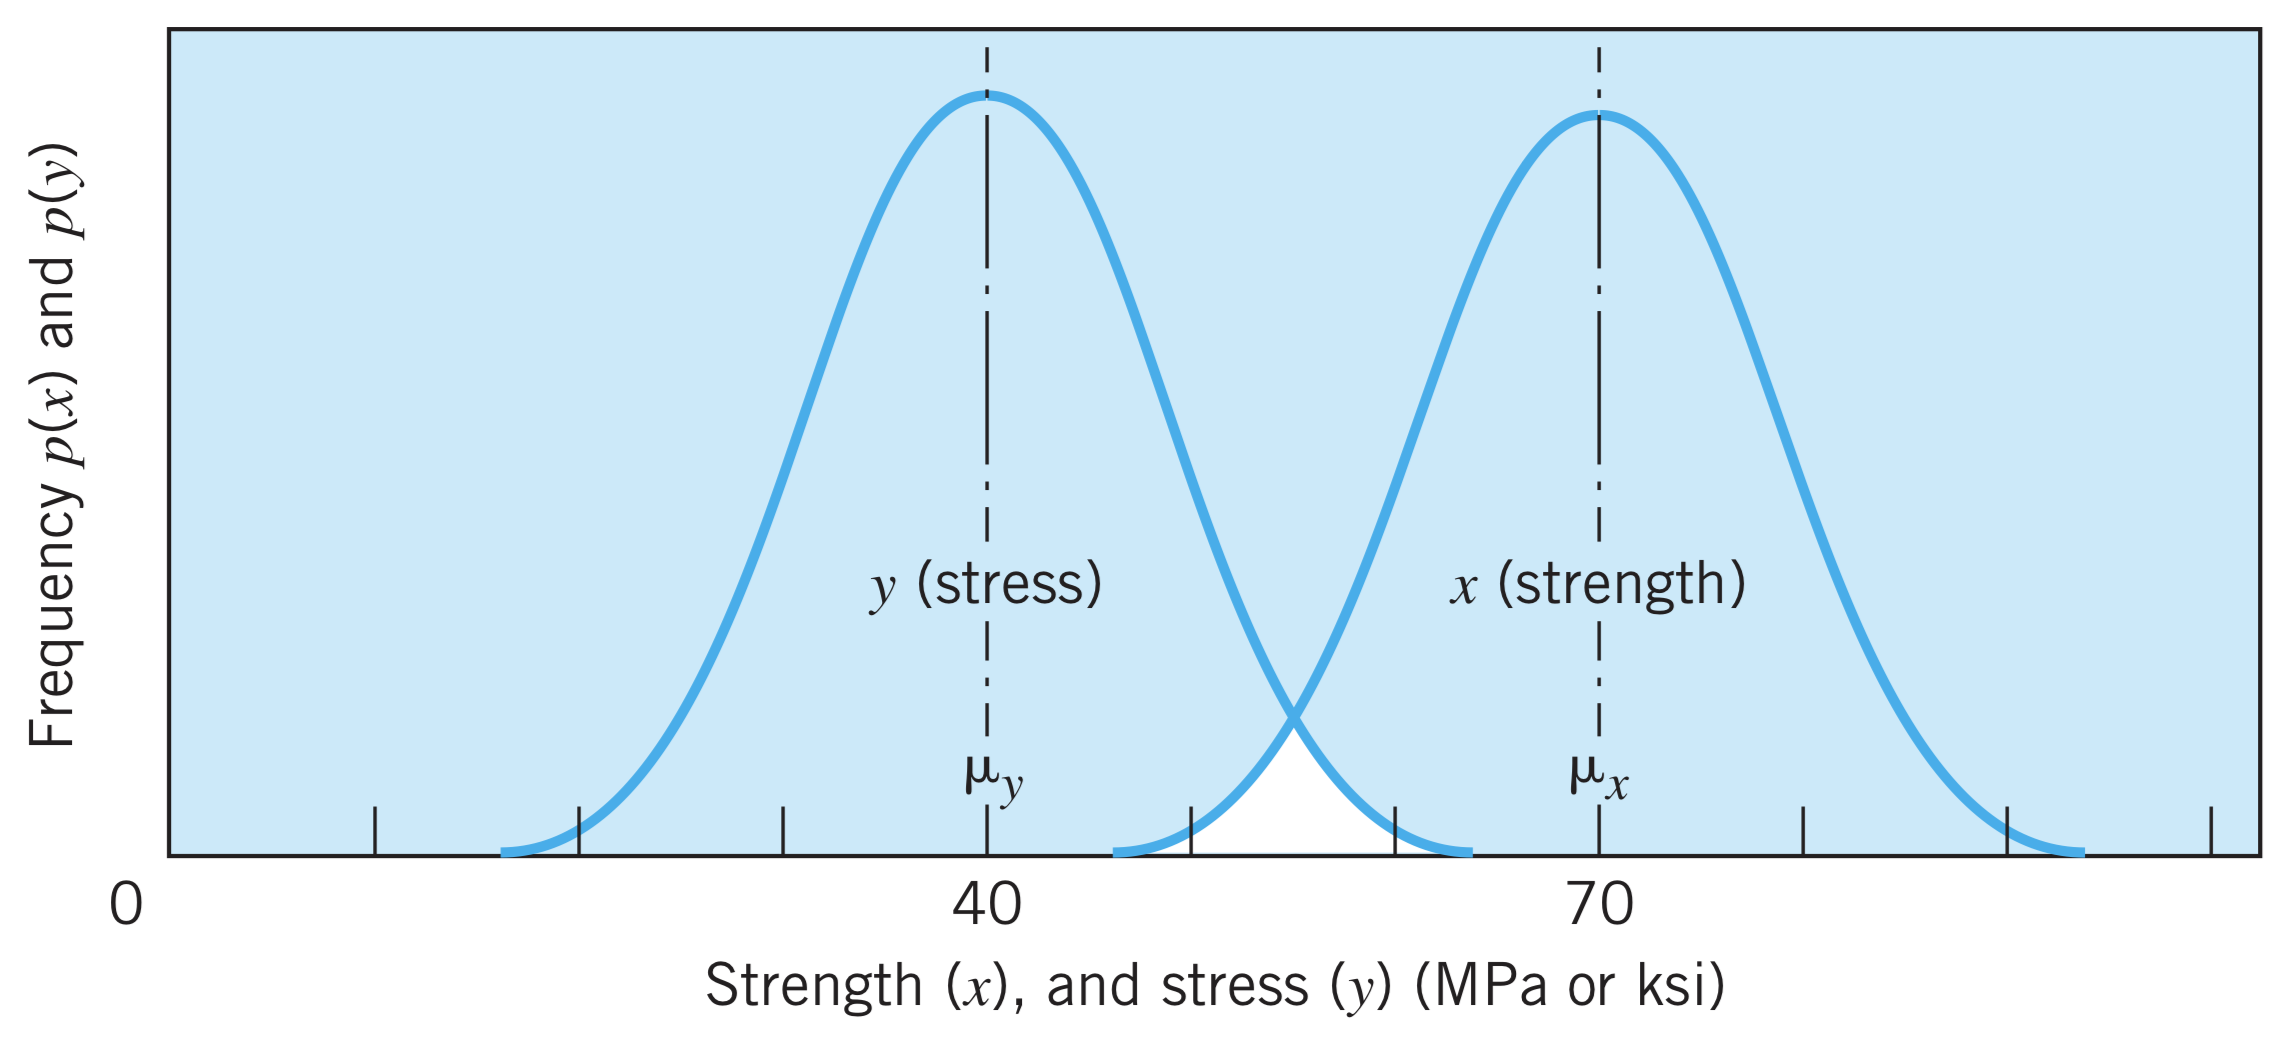
\includegraphics[width=0.9\textwidth]{A1_safety_factor/stress-strength-dist.png}
  \caption[The probability distributions of stress and strength showing substantial overlap]{The probability distributions of stress and strength showing substantial overlap~\cite{juvinall1983}}
  \label{fig-prob-dist}
\end{figure}

Based on \cref{fig-prob-dist}, we may modify the safety factor Equation~\ref{equ-safety-1} to account for this overlap between stress and strength as follows~\cite{joseph2001}:

\begin{equation}
  N_R = N \bigg( \frac{1-a\gamma_s}{1+a\gamma_\sigma} \bigg) > 1
  \label{equ-safety-2}
\end{equation}

\noindent where:

\begin{description}
  \item[$N_R$] is the safety factor based on reliability
  \item[$N$] is the central safety factor based on mean or expected values (Equation~\ref{equ-safety-1})
  \item[$\gamma_s$] is the coefficient of variation of the strength value (published or estimated)
  \item[$\gamma_\sigma$] is the coefficient of variation of the stress value (estimated)
  \item[$a$] is the number of standard deviations to produce the desired confidence level \pref{tbl-a}
\end{description}

\begin{table*}
  \center{}
  \small
  \begin{tabular}{l r r r r r r r r}
    \toprule
    $a$ & 0 & 1.65 & 2.33 & 3 & 3.08 & 3.62 & 4.42 & 4.89 \\
    \midrule
    Reliability & 50\% & 95\% & 99\% & 99.87\% & 99.9\% & 99.99\% & 99.999\% & 99.9999\% \\
    Failure Rate & $\frac{1}{2}$ & $\frac{1}{20}$ & $\frac{1}{100}$ & $\frac{1}{769}$ & $\frac{1}{1000}$ & $\frac{1}{10000}$ & $\frac{1}{100000}$ & $\frac{1}{1000000}$ \\
    \bottomrule
  \end{tabular}
  \vspace{2em}
  \caption{Values for $a$}
  \label{tbl-a}
\end{table*}

Notice that Equation~\ref{equ-safety-2} is a relatively simple modification of the definition of central safety factor (Equation~\ref{equ-safety-1}) that compares the highest expected stress against the lowest expected strength based on the specified level of reliability.

\begin{figure}
  \centering
  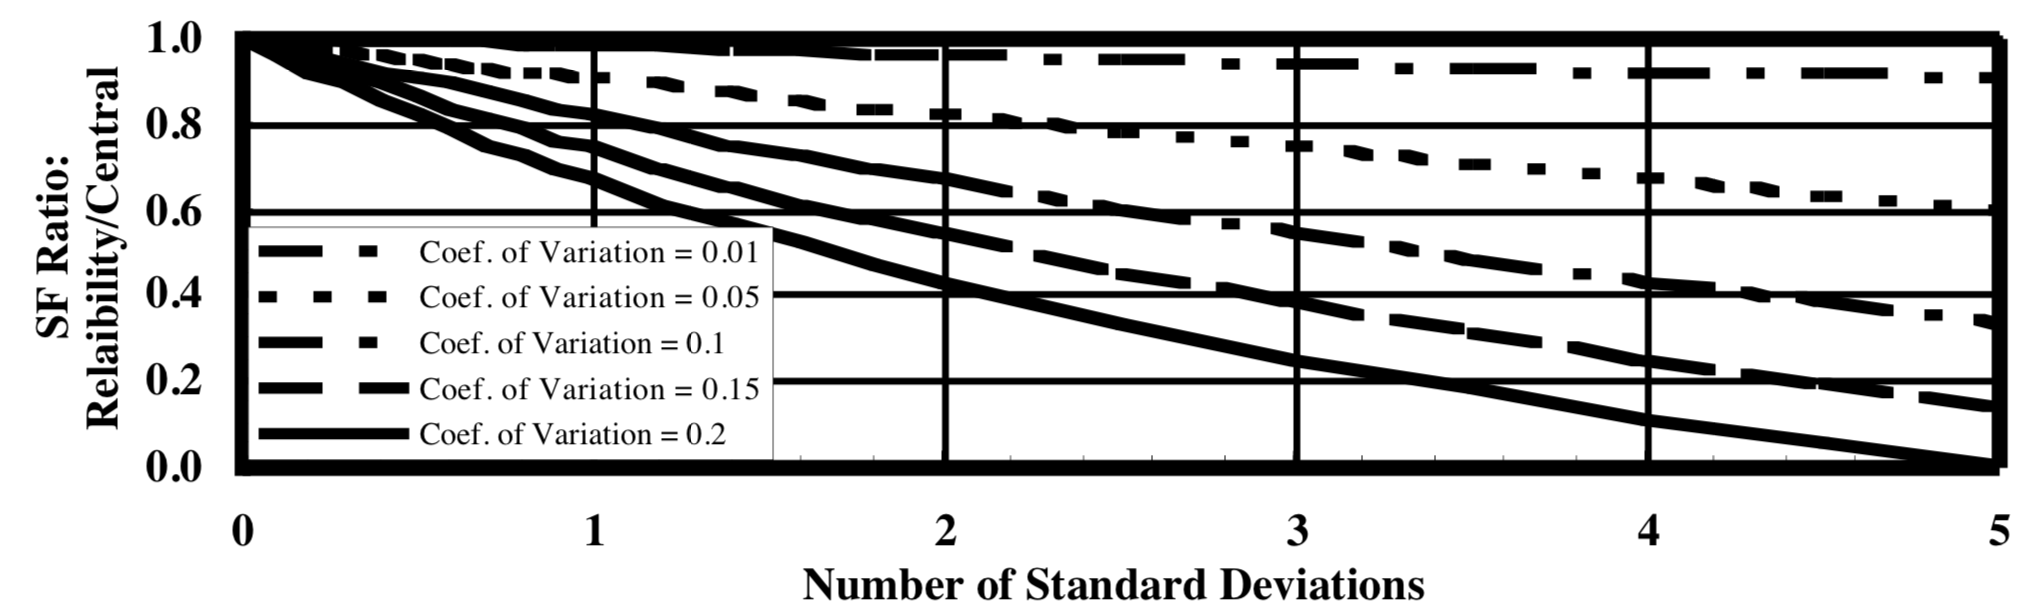
\includegraphics[width=\textwidth]{A1_safety_factor/sf-ratio.png}
  \caption{Ratio of the reliability safety factor to the central safety factor}
\end{figure}

\subsection{The Visodic Safety Factor Model}

Joseph P. Visodic developed and published recommendations for minimum central safety factor values in 1948 which were based on cumulative experience~\cite{joseph2001}\cite{juvinall1983}. These are presented in Table~\ref{tbl-visodic}. Safety factors for ductile materials are based on yield strength. Safety factors for brittle materials are based on ultimate strength and are twice the recommended values for ductile materials. Safety factors for primarily cyclic loading are based on endurance limit. Impact loads require a safety factor of at least 2 multiplied by an ``impact factor'', usually in the range of 1.1 to 2.

\begin{table}
    \footnotesize
    \centering
    \begin{tabular}{p{0.15\textwidth} p{0.15\textwidth} p{0.15\textwidth} p{0.15\textwidth} p{0.15\textwidth}}
      \toprule
        Safety Factor & Knowledge of Loads & Knowledge of Stress & Knowledge of Material & Knowledge of Environment \\
      \midrule
        1.2-1.5 & Accurate & Accurate & Well Known & Controllable \\
        1.5-2.0 & Good & Good & Well Known & Constant \\
        2.0-2.5 & Good & Good & Average & Ordinary \\
        2.5-3.0 & Average & Average & Less Tried & Ordinary \\
        3.0-4.0 & Average & Average & Untried & Ordinary \\
        3.0-4.0 & Uncertain & Uncertain & Better Known & Uncertain \\
      \bottomrule
    \end{tabular}
  \caption[Recommended central safety factors for ductile materials based on yield strength]{Recommended central safety factors for ductile materials based on yield strength~\cite{joseph2001}}
  \label{tbl-visodic}
\end{table}

\subsection{The Norton Safety Factor Model}

Robert L. Norton \mycite{robert2006} stated ``Clearly, where human safety is involved, high values of (safety factor) are justified''. His overall safety factor value is a combination of a safety factor based on material properties, one based on engineering model accuracy, and one based on expected service environment, as follows:

\begin{eqnarray}
  N_{\text{ductile}} \geq \max(N_1, N_2, N_3); \text{ based on yield strength} \\
  N_{\text{brittle}} \geq 2\times\max(N_1, N_2, N_3); \text{ based on ultimate strength}
\end{eqnarray}

\noindent Where $N_1, N_2$ and $N_3$ are selected from Table~\ref{tbl-norton}.

\begin{table}
  \centering
  \small
  \begin{tabular}{p{0.1\textwidth} p{0.25\textwidth} p{0.25\textwidth} p{0.25\textwidth}}
    \toprule
      Safety Factor & $N_1$ & $N_2$ & $N_3$ \\
      & Material Properties (from tests) & Stress/Load Model Accuracy & Service Environment \\
    \midrule
    1.3 & Well known/characterized & Confirmed by testing & Same as material test conditions \\
    2 & Good approximation & Good approximation & Controlled, room-temperature \\
    3 & Fair approximation & Fair approximation & Moderately challenging \\
    5+ & Crude approximation & Crude approximation & Extremely challenging\\
    \bottomrule
  \end{tabular}
  \label{tbl-norton}
  \caption[Recommended central safety factors for ductile materials based on yield strength]{Recommended central safety factors for ductile materials based on yield strength \cite{robert2006}}
\end{table}

\subsection{The Pugsley Safety Factor Model}

Please see \cref{sec:DF}.

\subsection{Misc. Safety Factor Models}

Lipson and Juvinall~\cite{lipson1963} presented the safety factor recommendation shown in tables 4 and 5, which were based on cumulative experience. In order to compare the values in these tables with the values in the previous tables, let us assume that the yield strength of hot rolled steel is half of the ultimate strength, therefore the safety factors can be cut in half (except for those listed for cast iron, which is brittle).

\begin{table}
  \centering
  \small
  \begin{tabular}{p{0.3\textwidth} c c}
    \toprule
    Kind of Load & Steel (Ductile) & Cast Iron (Brittle) \\
    \midrule
    Dead (static) load & 5 & 6 \\
    Repeated, gradually applied in one direction with mild shock & 6 & 10 \\
    Repeated, gradually applied in reversed directions with mild shock & 8 & 15 \\
    Shock load & 12 & 20 \\
    \bottomrule
  \end{tabular}
  \caption{recommended safety factors based on ultimate strength}
\end{table}

\subsection{Discussion and Recommendations}

The value of a central safety factor (Equation~\ref{equ-safety-1}) should not be less than two (2) for most structural applications and should routinely be set at three (3). Low safety factors are justified only where extensive physical testing of both materials and structural systems is done. Low safety factors also require routine periodic inspection and maintenance of the system if it is to have a useable life of more than a few years in an ordinary service environment. Uncertainty in loading, uncertainty in material properties, foreseeable abuse, and challenging service environments demand higher values of the safety factor. A long service life also requires a larger value of safety factor. High reliability applications require systems with a larger central safety factor value.

The reliability safety factor (Equation~\ref{equ-safety-2}) accommodates lower values than the central safety factor (Equation~\ref{equ-safety-1}) for the same probability of failure. Shigley~\cite{joseph2001} feels that given well known values and a reasonable reliability level (95\% or higher) safety factor values between 1.3 and 2.0 are adequate. Again, lower safety factor values require physical testing, a predictable service environment, and periodic inspection and maintenance.

Brittle\marginnote{Brittle Materials} materials require a higher safety factor than ductile materials because brittle failure is abrupt and not preceded by yielding. The consensus in the literature is that the safety factor for brittle materials should be at least twice that used for ductile materials and should be based on ultimate strength.

Service\marginnote{Service Loads} loads due to expected normal use and foreseeable abuse are usually difficult to establish. Well characterized loads justify a lower minimum safety factor value, while uncertain loads require a larger value.

Cyclic loading\marginnote{Cyclic Loading} induces fatigue failure in structural components. The safety factor for primarily cyclic loading should be based on the endurance limit rather than on yield or tensile strength. Well characterized cyclic loads justify a lower minimum safety factor value, while uncertain loads should have a larger value.

Impact\marginnote{Impact Loading} (shock) loading induces very high transient stresses in structural components that can precipitate failure. Therefore the safety factor for impact loading should be at least 2.0, and 1.5 to 2.5 times that used for static (dead) loads. The greater the impact force, the higher the safety factor needed.

The consequences of system failure must also be considered in the selection of a minimum safety factor value. If human life and health are not at risk and potential property damage is limited to the system itself, then the minimum safety factor value may be lowered a little. However if human life and health are at risk and/or potential property damage caused by system failure is substantial, then a higher minimum safety factor value is required. These are the situations in which failure precipitates liability litigation and therefore a higher safety factor should be viewed as relatively cheap liability insurance.

The service life of the system is important in the selection of a minimum safety factor value. A short expected service life justifies a lower minimum safety factor value, while a long expected service life demands a higher value.

The service environment also affects the selection of a minimum safety factor value. A controlled indoor environment may accommodate a lower minimum safety factor value, while a challenging environment involving temperature extremes, corrosion, earthquake, occasional high winds, etc. needs a substantially larger value.

\begin{table}
    \centering
    \small
    \begin{tabular}{p{0.5\textwidth} c c c}
      \toprule
        Test Case & Visodic & Norton & Pugsley \\
      \midrule
        \textbf{Commercial aerospace structure:} Very well tested materials and structures. Well Characterized loads. Predictable service environment. Periodic inspection and maintenance throughout long life. Failure usually results in high risk to many human lives. (A SF of 1.5 is expected.)
        & 1.2-1.5
        & 1.3
        & 1.4
        \\
        \textbf{Trailer hitch coupler:} Defined maximum loads by class. Occasional service loads 2-3 times defined maximums. Corrosive environment. Cyclic and impact loading. Very little inspection and maintenance during moderately long life. Failure may result in high risk to human life.
        & 4.0-6.0
        & 4.0
        & 4.0
        \\
        \textbf{Large utility power transformer:} Well defined maximum loads. Occasional service loads 1-2 times normal. Cyclic and impact loading. Predictable but challenging service environment. Periodic inspection and maintenance throughout very long life. (A SF of 5 is customary.)
        & 3.8-5.0
        & 4.0
        & 3.8
        \\
      \bottomrule
    \end{tabular}
  \caption{a comparison of safety factor models}
\end{table}


\clearpage
\section{Polygonal Action in Chain Drives}

The speed of a chain\marginnote{Abstract \citep{mahalingam1958}} is subject to periodic fluctuations, even for a constant speed of the driving sprocket, due to the fact that a chain lying on a sprocket forms a polygon rather than a circle. It is shown that the dynamic loading of the chain due to this ``polygonal action'' is similar to that of a simple forced vibration where, beyond a certain critical speed, higher speeds produce lower dynamic loads.

\marginnote{notation} 
\begin{description}
\item[$R$] Radius of sprocket (to center of chain pin)
\item[$T$] Number of teeth in sprocket
\item[$n$] Mean speed of sprocket (\si{\radian\per\second})
\item[$r$] Period of tooth engagement $\left(\frac{2\pi}{nT}\right)$
\item[$p$] circular frequency of tooth engagement $\left(nT\right) (\si{\radian\per\second})$
\item[$I$] Moment of inertia of driven system about axis of rotation
\item[$k$] Longitudinal stiffness of unsupported length of chain
\end{description}

The suffixes 1 and 2 refer to the driving and driven system, respectively.

When\marginnote{Introduction} the driving sprocket of a chain drive runs at constant speed, the speed of the chain itself is not constant but is subject to periodic fluctuations. This fluctuation, which is caused by the fact that the chain when wrapped on a sprocket forms a polygon rather than a circle, is known as polygonal action.

One effect of polygonal action is to produce a periodic variation in the velocity ratio of the drive, and if the frequency of this variation coincides with a resonant frequency of the system, large stresses may occur. In this respect the chain drive is similar to a Hooke's joint. Another product of the geometry of the chain drive is impact. The cause of impact is the difference in the velocities of the point on the roller and the point on the sprocket that come into contact. Polygonal action is continuous being characterized by small fluctuations, while impact represents a sharp blow of short duration. At high chain speeds the effects of impact are very complex; each impact sets up a train of travelling waves which, after reflection at the sprockets, combine with the next train and so on. The resultant ``surge'' of the chain completely predominates the dynamic effects of polygonal action. It would therefore be very difficult to separate the two factors at high speeds.

At low speeds, however, the impulsive loads are small and, owing to the longer interval between impacts, the travelling waves are damped out. Then under certain conditions the dynamic load due to polygonal action is of great importance and an analysis of this factor is made below.

Some aspects of polygonal action have been discussed in recent years. In a paper on the use of chain drives in marine diesel engines, Bremer~\cite{bremer1947} referred to the fluctuation of the chain speed and to minimize it he recommended sprockets of at least about 30 teeth. The variation of the angular speed of the driven sprocket was studied by Morrison~\cite{morrison1952}. In his analysis the drive was considered as being equivalent to a series of four-bar linkages, each acting for a period equal to the period of tooth engagement.

The analysis given below deals with the dynamic load in the chain strand, taking into consideration the elasticity of the chain and the moment of inertia of the driven system. It is shown that the effect of polygonal action is similar to that of a forced vibration.

In\marginnote{Analysis} the following analysis it will be assumed that the driving sprocket runs at a constant speed of $n_1$ \si{\radian\per\second}. The reference axes, taken at $O_1$, will be parallel and perpendicular to the direct common tangent to the pitch circles of the sprockets. The change of slope of the chain will be neglected.


In \cref{fig-poly-1}, $A_1$ and $A_2$ represent the pins that are articulating and therefore $O_1A_1A_2O_2$ represents the equivalent four-bar mechanism. Angles $B_1O_1C_1$ and $B_2O_2C_2$ represent the range of operation of the linkage. The exact formula for $O_2$, assuming $A_1A_2$ to be rigid, as given in \ref{eq-poly-3} is extremely cumbersome and an approximate value may be obtained as follows:

\begin{equation}
  \text{Speed of Chain} \simeq n_1R_1\sin\theta_1 
\end{equation}

\noindent{} Hence,

\begin{equation}
  \dot{\theta_2} \simeq n_1\frac{R_1\sin\theta_1}{R_2\sin\theta_2}
\end{equation}

In practice, this method usually gives a high degree of accuracy because the angles $B_1O_1C_1$ and $B_2O_2C_2$ are small and the change in the slope of $A_1A_2$ is negligible.

\begin{figure}[th!]
  \centering
  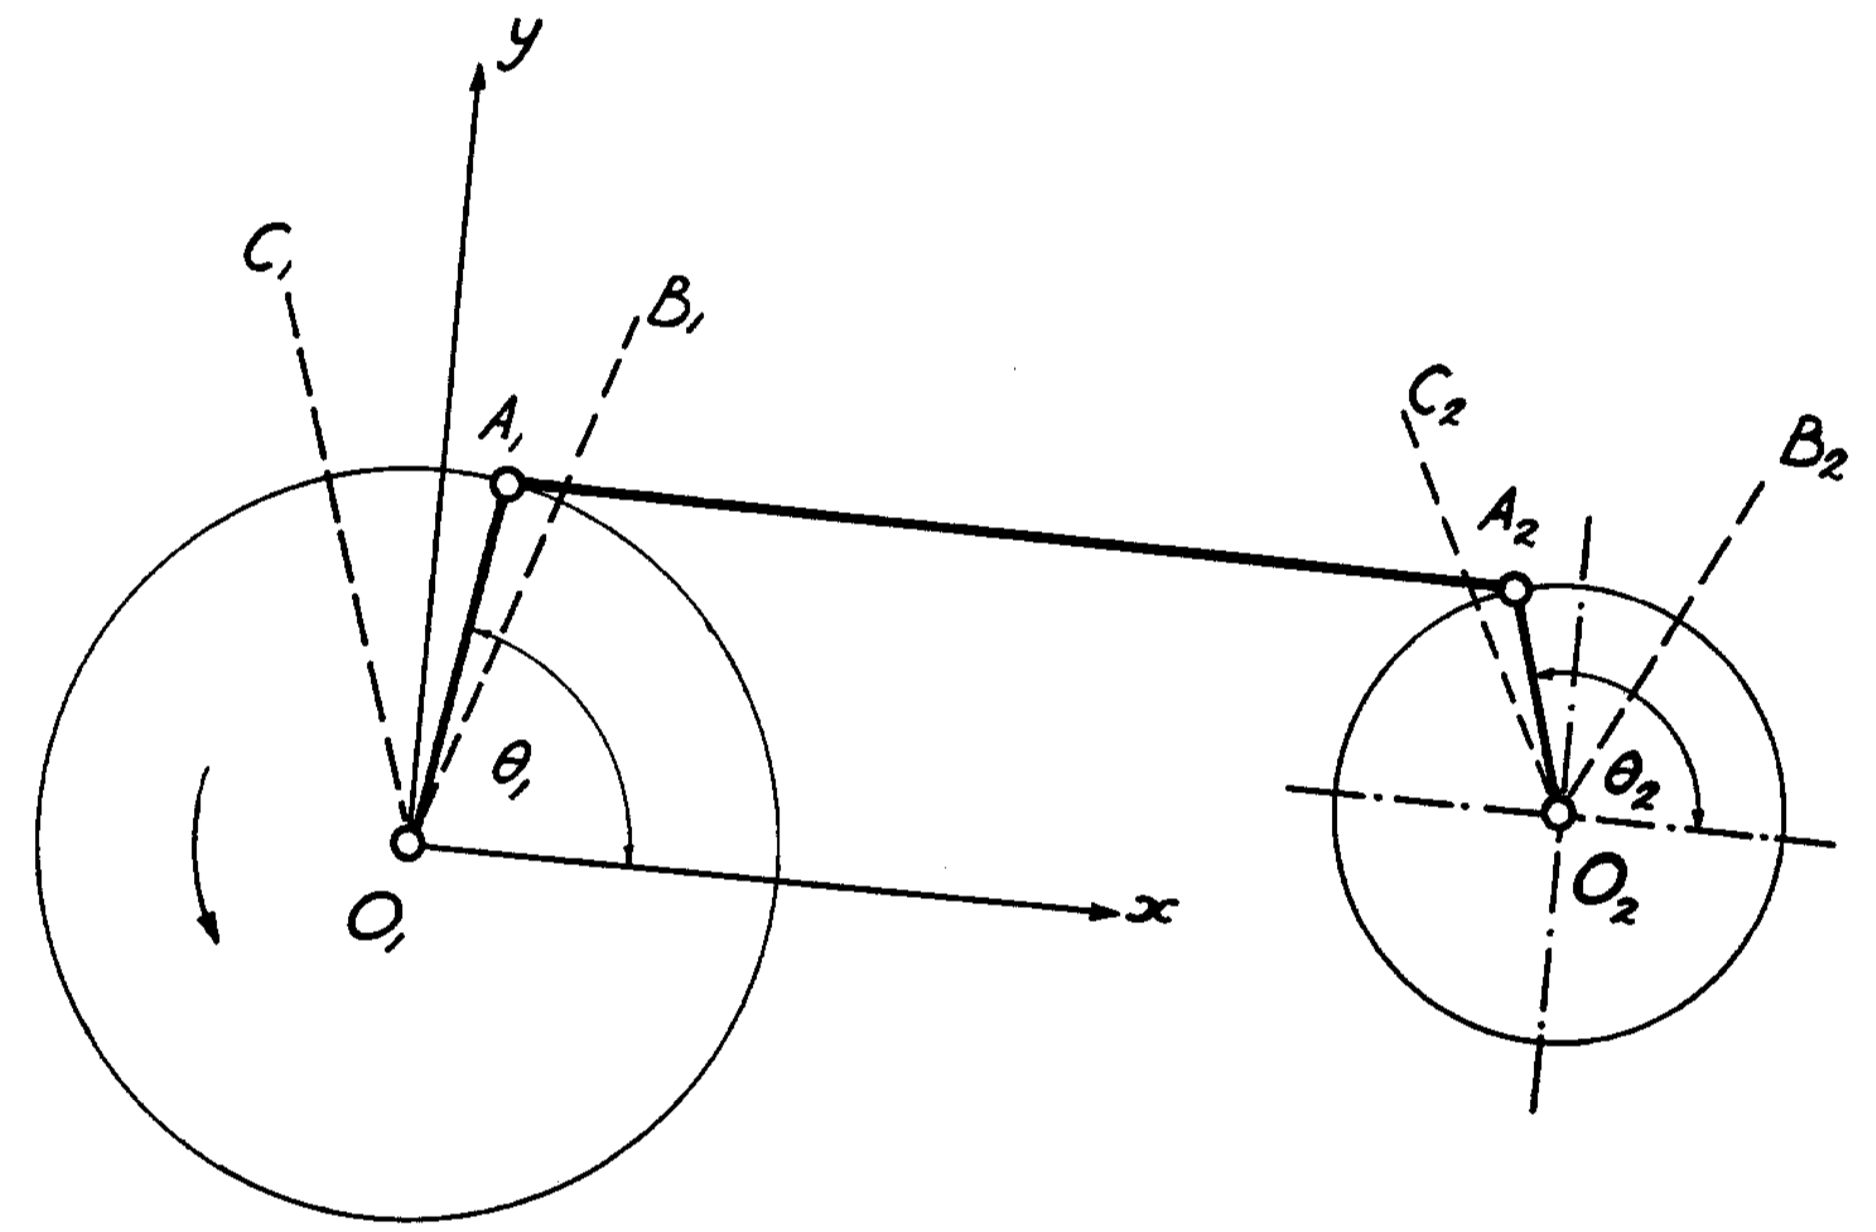
\includegraphics[width=0.9\textwidth]{A2_polygonal_action/fig1.png}
  \caption{equivalent four-bar linkage in chain drive}
  \label{fig-poly-1}
\end{figure}

When two equal sprockets are used at a distance apart equal to an integral multiple of the pitch, then $R_1\sin\theta_1$ is always equal to $R_2\sin\theta_2$,and $\dot{\theta}_2$ is constant. In all other cases $\dot{\theta}_2$ will be subject to small fluctuations.

The elasticity of the chain will now be considered. Since each four-bar linkage operates for a period $\tau=\frac{2\pi}{n_1T_1}=\frac{2\pi}{n_2T_2}$ the quantity $R_1\sin\theta_1$ is a function of period $\tau$ and can therefore be expressed as a Fourier series. If we include only the fundamental harmonic term of the series, then it may be shown that

\begin{equation}
    R_1\sin\theta_1 \simeq R_1\frac{T_1}{\pi}\sin\frac{\pi}{T_1}\left[1-\frac{2}{T_1^2-1}\cos pt\right]
    \label{eq-poly-2}
\end{equation}

where $p=n_1T_1=n_2T_2$, and $t$ represents time.

In most power transmitting sprockets the number of teeth is never less than about 15 and therefore the coefficient $\frac{2}{T_1^2-1}$ may be regarded as a small quantity.

Equation~\ref{eq-poly-2} may be written in a simpler form as:

\begin{equation}
  R_1\sin\theta_1 \simeq a_0 + a_1\cos pt
\end{equation}

The speed of $A_1$ is then given by:

\begin{equation}
  -\dot{x}_1 \simeq n_1\left(a_0+ a_1\cos pt\right)
\end{equation}

and by integration:

\begin{equation}
  -x_1 \simeq n_1\left(a_0t+ \frac{a_1}{p}\sin pt\right) + A
  \label{eq-poly-3}
\end{equation}

where $A$ is the constant of integration. In a similar manner it may be shown that:

\begin{equation}
  R_2\sin\theta_2 \simeq Na_0+\frac{a_1}{N}\cos (pt-\alpha)
  \label{eq-poly-4}
\end{equation}

where:

\begin{description}
\item[$\alpha$] a ``phase angle'' corresponding to the fractional pitch in direct common tangent to the pithc circles
\item[$N$] speed ratio $\frac{T_2}{T_1}=\frac{R_2}{R_1}\frac{\frac{T_2}{\pi}\sin\frac{\pi}{T_2}}{\frac{T_1}{\pi}\sin\frac{\pi}{T_1}}$
\end{description}

Equation~\ref{eq-poly-4} has been derived on the assumption that the speed of the driven sprocket is constant. The speed is in fact subject to small fluctuations but it may be shown that the error involved in Equation~\ref{eq-poly-4} is negligible.

Equation~\ref{eq-poly-4} may be written

\begin{equation}
  R_2\sin\theta_2\simeq Na_0+\frac{b_1}{N}\cos pt + \frac{c_1}{N}\sin pt
  \label{eq-poly-5}
\end{equation}

where:

\begin{itemize}
\item $b_1=a_1\cos\alpha$
\item $c_1=a_1\sin\alpha$
\end{itemize}

Let the speed of $A_2$ be given by:

\begin{equation}
  -\dot{x}_2 \simeq \frac{n_1}{N}\left[Na_0+\frac{l_1}{N}\cos pt +\frac{m_1}{N} \sin pt\right]
  \label{eq-poly-6}
\end{equation}

where $l_1$, $m_1$ are constant to be determined.

Integrating and substituting boundary conditions

\begin{equation}
  -\dot{x}_2 \simeq \frac{n_1}{N}\left[Na_0t+\frac{l_1}{pN}\sin pt +\frac{m_1}{pN} \cos pt\right] + A + l
\end{equation}

Now $\dot{\theta}_2 \simeq \frac{-\dot{x}_2}{R_2\sin\theta_2}$ and substituting from \ref{eq-poly-5} and \ref{eq-poly-6} and noting that $b_1$ and $c_1$ are small quantities we get:

\begin{equation}
  \dot{\theta}_2 \simeq \frac{n_1}{N}\left[ 1 + \frac{l_1-b_1}{N^2a_0}\cos pt + \frac{m_1-c_1}{N^2a_0} \sin pt \right]
\end{equation}

This gives

\begin{equation}
  \ddot{\theta}_2 = \frac{N1p}{N^3a_0}\left[(m_1-c_1)\cos pt - (l_1-b_1)\sin pt \right]
\end{equation}

For the oscillation of the driven system about its axis of rotation, the equation of motion is:

\begin{equation}
  I\ddot{\theta}_2 = k(x_1+l-x_2)R_2\sin\theta_2=0
\end{equation}

where $I=$ moment of inertia of driven system about axis of rotation and $k=$ longitudinal stiffness of chain.

Substituting for $\ddot{\theta}_2$, $x_2$, $x_1$ and $R_2\sin\theta_2$ we get

\begin{equation}
  \left[p^2(m_1-c_1)-\omega^2m_1 \right]\cos pt + \left[\omega^2(l_1-a_1N^2)-p^2(l_1-b_1) \right]\sin pt = 0
\end{equation}

where $\omega = \left(\frac{kN^2a_0^2}{I}\right)^\frac{1}{2}$

Since this equation is to be satisfied for all $t$, we get

\begin{equation}
  m_1 = \frac{c_1}{1-\frac{\omega^2}{p^2}}
\end{equation}

and

\begin{equation}
  l_1=\frac{b_1-a_1\frac{N^2\omega^2}{p^2}}{1-\frac{\omega^2}{p^2}}
\end{equation}

\begin{equation}
\text{Dynamic load in chain} =k(x_1+l-x_2)
\end{equation}

\begin{equation}
=\frac{k}{T_1}\left[\left(\frac{l_1}{N^2}-a_1\right)\sin pt - \frac{m_1}{N^2}\cos pt\right]
\end{equation}

Substituting for $l_1$ and $m_1$ the maximum dynamic load is given by

\begin{equation}
  P=\frac{k}{T_1}\left[\left(\frac{b_1}{N^2}-a_1\right)^2+\left(\frac{c_1}{N^2}\right)^2\right]^\frac{1}{2} \frac{1}{1-\frac{\omega^2}{p^2}}
\end{equation}


This shows that the dynamic effect of polygonal action is similar to that of a forced vibration and that large forces may develop when $p$, the circular frequency of tooth engagement, is equal to $\omega$, the natural circular frequency of the system.

Putting

\begin{itemize}
\item $b_1=a_1\cos\alpha$
\item $c_1=a_1\sin\alpha$
\end{itemize}

we get

\begin{equation}
  \begin{split}
  P &\propto \frac{a_1^2}{N^4}\left[\left(\cos\alpha-N^2\right)^2 + \sin^2\alpha\right] \\
  &\propto \frac{a_1^2}{N^4}\left(1-2N^2\cos\alpha+N^4\right)
  \end{split}
\end{equation}

This shows that for a given speed ratio $N$, the dynamic load $P$ is

\begin{itemize}
\item[i] a minimum when $\alpha=0$, that is, integral number of pitches in the direct common tangent.
\item[ii] a maximum when $\alpha=\pi$, that is, an odd number of half pitches in the direct common tangent.
\end{itemize}

As can be expected, the dynamic load is zero when $N = 1$ and $\alpha = 0$, that is, equal sprockets at a distance apart equal to an integral multiple of the pitch.

It is also possible for resonance to occur at half the critical speed, being excited by the second harmonic, but the dynamic load due to this is likely to be small.






\end{document}